%----------------------------------------------------------------------------------------
%    PACKAGES AND THEMES
%----------------------------------------------------------------------------------------

\documentclass[aspectratio=169,xcolor=dvipsnames]{beamer}

\input{slides/utils/preamble}
\input{slides/utils/custom-commands}
\usetikzlibrary{spy}

%----------------------------------------------------------------------------------------
%    TITLE PAGE
%----------------------------------------------------------------------------------------

\title{Deep Learning}
\subtitle{Introdução a Redes Convolucionais}

\author{Lucas Silveira Kupssinskü}

\institute
{
    Machine Learning Theory and Applications Laboratory \\
    PUCRS
}
\date{\mespor de \the\year}

%----------------------------------------------------------------------------------------
%    PRESENTATION SLIDES
%----------------------------------------------------------------------------------------

\begin{document}

\begin{frame}
    \titlepage
\end{frame}

\begin{frame}{Overview}
    \tableofcontents
\end{frame}

%========================================================================
\section{Motivação}
%========================================================================

\begin{frame}{Motivação Histórica}
\begin{columns}
    \begin{column}{.6\linewidth}
        \begin{itemize}
            \item David Hubel e Torsten Wiesel realizaram experimentos implantando eletrodos no córtex visual de gatos\footfullcite{hubel1962receptive}.
            \item Aparentemente o processamento começa identificando padrões simples, como arestas.
            \begin{itemize}
                \item \href{https://www.youtube.com/watch?v=jw6nBWo21Zk}{Vídeo}
            \end{itemize}
            \item Camadas seguintes combinam esses padrões em estruturas mais complexas.
        \end{itemize}
    \end{column}
    \begin{column}{.4\linewidth}
        \centering
        \includegraphics[width=\linewidth]{slides/img/02-cnn/hubel_wiesel.jpeg}
    \end{column}
\end{columns}
\end{frame}

\begin{frame}{Redes Convolucionais}
\begin{itemize}
    \item São redes que incluem operações de convolução.
    \begin{itemize}
        \item Usadas principalmente em imagens.
    \end{itemize}
    \item Criadas em 1989 por Yann LeCun, com a LeNet\footfullcite{lecun1989backprop}.
    \item Explodiram em popularidade após 2012, com a AlexNet\footfullcite{krizhevsky2012imagenet}.
    \begin{itemize}
        \item Treinamento em GPUs.
        \item Mais dados.
        \item Mais poder computacional.
    \end{itemize}
\end{itemize}
\end{frame}

\begin{frame}{Problemas com MLP}
\begin{columns}[T]
    \begin{column}{.52\linewidth}
        Imagens têm \textbf{três propriedades} que sugerem o uso de
        arquiteturas específicas:
        \medskip

        \only<1>{%
          \textbf{1.~Alta dimensionalidade}
          \begin{itemize}
            \item Uma imagem $512\times 512$ resulta em $262.144$ pixels.
            \item Com 100 unidades na primeira camada oculta de um MLP,
            teríamos $26.214.400$ pesos.
            \item Em \texttt{float32} (4 bytes por peso), $\approx 100$ MB
            \textbf{só} na primeira camada.
          \end{itemize}}
        \only<2>{%
          \textbf{2.~Alta coesão espacial}
          \begin{itemize}
            \item Pixels próximos têm valores \textbf{altamente
            correlacionados} (veja o \textit{zoom} ao lado).
            \item Uma mesma característica (ex.: uma orelha) pode aparecer
            em \textbf{vários locais} da imagem.
          \end{itemize}}
        \only<3>{%
          \textbf{3.~Semântica estável a transformações geométricas}
          \begin{itemize}
            \item Translações, rotações e deformações \textbf{não mudam}
            o conteúdo: continua sendo um gato.
          \end{itemize}}
    \end{column}
    \begin{column}{.46\linewidth}
        \centering
        \only<1>{%
          \includegraphics[height=5.0cm]{slides/img/02-cnn/mlp_diagram.png}\\[3pt]
          {\scriptsize MLP totalmente conectado: milhões de pesos.}}
        \only<2>{%
          \begin{tikzpicture}[spy using outlines={rectangle, magnification=4,
              size=2.3cm, connect spies}]
            \node[inner sep=0] (dog)
              {\includegraphics[width=4.3cm]{slides/img/02-cnn/mlp_dog.jpeg}};
            \spy[BrickRed, very thick] on (0,-0.55) in node at (3.05,-0.2);
          \end{tikzpicture}\\[3pt]
          {\scriptsize Vizinhança quase uniforme $\to$ valores semelhantes.}}
        \only<3>{%
          \includegraphics[height=2.0cm]{slides/img/02-cnn/mlp_cat.jpeg}\hspace{0.25cm}%
          \rotatebox{15}{\includegraphics[height=2.0cm]{slides/img/02-cnn/mlp_cat.jpeg}}\\[6pt]
          {\scriptsize Original e rotacionado: ainda é ``gato''.}}
    \end{column}
\end{columns}
\end{frame}

\begin{frame}{Camadas Convolucionais}
\begin{block}{Camadas convolucionais trazem diversos benefícios:}
\begin{itemize}
    \item Processam regiões da imagem separadamente, compartilhando pesos.
    \item Usam menos parâmetros do que camadas totalmente conectadas.
    \item Exploram a correlação entre pixels próximos.
    \item Não precisam reaprender padrões em locais diferentes da imagem.
\end{itemize}
\end{block}
\end{frame}

%========================================================================
\section{Invariância e Equivariância}
%========================================================================

\begin{frame}{Invariância}
\begin{itemize}
    \item Uma função $f$ aplicada a uma imagem $\mathbf{X}$ é dita \textbf{invariante} a uma transformação $t$ se:
\end{itemize}
\begin{equation*}
    f\bigl[t[\mathbf{X}]\bigr] = f[\mathbf{X}]
\end{equation*}
\begin{itemize}
    \item Ou seja, independente da transformação aplicada na entrada, o resultado é o mesmo.
    \item Exemplo: classificar a imagem como ``gato'' não deveria depender de o gato estar à esquerda ou à direita do quadro.
\end{itemize}
\end{frame}

\begin{frame}{Equivariância}
\begin{columns}[T]
    \begin{column}{.5\linewidth}
        \begin{itemize}
            \item Uma função $f$ aplicada a uma imagem $\mathbf{X}$ é dita \textbf{equivariante} a uma transformação $t$ se:
        \end{itemize}
        \begin{equation*}
            f\bigl[t[\mathbf{X}]\bigr] = t\bigl[f[\mathbf{X}]\bigr]
        \end{equation*}
        \begin{itemize}
            \item Ou seja, aplicar a transformação na entrada equivale a aplicá-la na saída.
            \item Exemplo: transladar a imagem de entrada deve resultar na mesma segmentação transladada.
        \end{itemize}
    \end{column}
    \begin{column}{.5\linewidth}
        \centering
        \includegraphics[width=\linewidth]{slides/img/02-cnn/equivariance_rooms.png}
    \end{column}
\end{columns}
\end{frame}

%========================================================================
\section{Convolução}
%========================================================================

\begin{frame}{Convolução 2D}
\begin{columns}[T]
    \begin{column}{.5\linewidth}
        \begin{itemize}
            \item A convolução transforma uma imagem de entrada $\mathbf{X}$ em uma imagem de saída $\mathbf{Z}$. Cada posição $(i,j)$ resulta de uma combinação linear de uma janela $3\times 3$ ao redor:
        \end{itemize}
        \begin{equation*}
            z_{i,j} = \sum_{m=1}^{3}\sum_{n=1}^{3} w_{m,n}\, x_{i+m-2,\, j+n-2}
        \end{equation*}
        \begin{itemize}
            \item Os pesos são \textbf{compartilhados} por toda a entrada.
            \item Esse conjunto de pesos é chamado de \textit{kernel} ou \textit{filtro}.
        \end{itemize}
    \end{column}
    \begin{column}{.5\linewidth}
        \centering
        \begin{tikzpicture}[every node/.style={font=\scriptsize}, scale=0.55]
            % Entrada 5x5 com janela 3x3 destacada
            \fill[black!22] (0.5,0.5) rectangle (2.0,2.0);
            \draw[step=0.5, gray!50] (0,0) grid (2.5,2.5);
            \draw[gray!50] (0,0) rectangle (2.5,2.5);
            \draw[thick, BrickRed] (0.5,0.5) rectangle (2.0,2.0);
            \node[font=\tiny, anchor=south] at (1.25,2.6) {Entrada $5\!\times\!5$};
            % Kernel 3x3 (grid colorido)
            \fill[PastelBlue2!25] (3.5,0.25) rectangle (5.0,1.75);
            \draw[step=0.5, gray!50, shift={(3.5,0.25)}] (0,0) grid (1.5,1.5);
            \draw[gray!50, shift={(3.5,0.25)}] (0,0) rectangle (1.5,1.5);
            \draw[thick, PastelBlue2!80!black] (3.5,0.25) rectangle (5.0,1.75);
            \node[font=\tiny, anchor=south] at (4.25,1.85) {Kernel};
            % Saida 3x3 com celula destacada
            \fill[black!22] (6.5,1.0) rectangle (7.0,1.5);
            \draw[step=0.5, gray!50] (6.0,0.5) grid (7.5,2.0);
            \draw[gray!50] (6.0,0.5) rectangle (7.5,2.0);
            \draw[thick, BrickRed] (6.5,1.0) rectangle (7.0,1.5);
            \node[font=\tiny, anchor=center] at (6.75,1.25) {$z_{ij}$};
            \node[font=\tiny, anchor=south] at (6.75,2.1) {Saída $3\!\times\!3$};
            % Setas
            \draw[->, BrickRed, thick] (2.55,1.25) -- (3.45,1.0);
            \draw[->, BrickRed, thick] (5.05,1.0) -- (6.45,1.25);
        \end{tikzpicture}
    \end{column}
\end{columns}
\end{frame}

\begin{frame}{Compartilhamento de Pesos}
\begin{columns}[T]
    \begin{column}{.5\linewidth}
        \begin{itemize}
            \item \textbf{O mesmo kernel} $w_{m,n}$ é deslizado por toda a entrada.
            \item O diagrama anterior mostrava apenas \emph{uma} aplicação do kernel; aqui ilustramos a aplicação em duas posições distintas.
            \item Para qualquer posição $(i,j)$:
            \begin{equation*}
                z_{i,j} = \sum_{m,n} w_{m,n}\, x_{i+m-2,\, j+n-2}
            \end{equation*}
            \item Não existem pesos próprios por $x_{i,j}$, os mesmos nove valores reaparecem em cada janela.
        \end{itemize}
    \end{column}
    \begin{column}{.5\linewidth}
        \centering
        \begin{tikzpicture}[every node/.style={font=\scriptsize}, scale=0.55]
            % Entrada 5x5 com duas janelas 3x3 destacadas
            \fill[BrickRed!25] (0.0,2.0) rectangle (1.5,3.5);
            \fill[PastelBlue2!35] (1.0,0.0) rectangle (2.5,1.5);
            \draw[step=0.5, gray!50] (0,0) grid (2.5,3.5);
            \draw[gray!50] (0,0) rectangle (2.5,3.5);
            \draw[thick, BrickRed] (0.0,2.0) rectangle (1.5,3.5);
            \draw[thick, PastelBlue2!80!black] (1.0,0.0) rectangle (2.5,1.5);
            \node[font=\tiny, anchor=south] at (1.25,3.6) {Entrada $5\!\times\!5$};
            % Kernel (mesmo, grid colorido)
            \fill[PastelBlue2!25] (3.5,1.0) rectangle (5.0,2.5);
            \draw[step=0.5, gray!50] (3.5,1.0) grid (5.0,2.5);
            \draw[gray!50] (3.5,1.0) rectangle (5.0,2.5);
            \draw[thick, PastelBlue2!80!black] (3.5,1.0) rectangle (5.0,2.5);
            \node[font=\tiny, anchor=south] at (4.25,2.6) {Mesmo kernel};
            % Saida 3x3 com duas celulas destacadas
            \fill[BrickRed!25] (6.5,2.0) rectangle (7.0,2.5);
            \fill[PastelBlue2!35] (7.5,0.5) rectangle (8.0,1.0);
            \draw[step=0.5, gray!50] (6.5,0.5) grid (8.0,2.5);
            \draw[gray!50] (6.5,0.5) rectangle (8.0,2.5);
            \draw[thick, BrickRed] (6.5,2.0) rectangle (7.0,2.5);
            \draw[thick, PastelBlue2!80!black] (7.5,0.5) rectangle (8.0,1.0);
            \node[font=\tiny, anchor=south] at (7.25,2.6) {Saída $3\!\times\!3$};
            % Setas
            \draw[->, BrickRed, thick] (1.55,2.75) -- (3.45,2.25);
            \draw[->, BrickRed, thick] (5.05,2.25) -- (6.45,2.25);
            \draw[->, PastelBlue2!80!black, thick] (2.55,0.75) -- (3.45,1.25);
            \draw[->, PastelBlue2!80!black, thick] (5.05,1.25) -- (7.45,0.75);
        \end{tikzpicture}
    \end{column}
\end{columns}
\end{frame}

\begin{frame}{\textit{Padding}}
\begin{columns}[T]
    \begin{column}{.45\linewidth}
        \begin{itemize}
            \item Como lidar com os extremos da entrada?
            \begin{itemize}
                \item \textit{Zero padding}: completar a entrada com zeros.
                \item \textit{Valid padding}: aplicar a convolução apenas onde o \textit{kernel} cabe inteiramente.
                \item Entrada ``circular'' ou periódica (pouco utilizado).
            \end{itemize}
        \end{itemize}
    \end{column}
    \begin{column}{.55\linewidth}
        \centering
        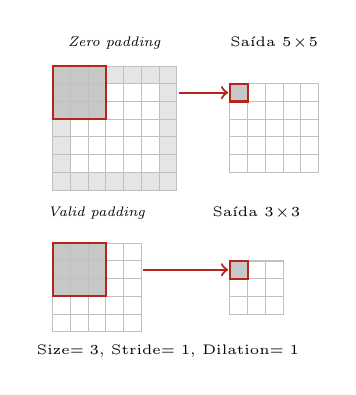
\begin{tikzpicture}[every node/.style={font=\scriptsize}, scale=0.45]
            % Zero padding: entrada 5x5 com borda de zeros (visual 7x7), saida 5x5
            \node[font=\tiny, anchor=south] at (1.75,3.7) {\textit{Zero padding}};
            \fill[black!10] (0,0) rectangle (3.5,3.5);
            \fill[white] (0.5,0.5) rectangle (3.0,3.0);
            \fill[black!22] (0.0,2.0) rectangle (1.5,3.5);
            \draw[step=0.5, gray!50] (0,0) grid (3.5,3.5);
            \draw[gray!50] (0,0) rectangle (3.5,3.5);
            \draw[thick, BrickRed] (0.0,2.0) rectangle (1.5,3.5);
            % Saida 5x5
            \fill[black!22] (5.0,2.5) rectangle (5.5,3.0);
            \draw[step=0.5, gray!50] (5.0,0.5) grid (7.5,3.0);
            \draw[gray!50] (5.0,0.5) rectangle (7.5,3.0);
            \draw[thick, BrickRed] (5.0,2.5) rectangle (5.5,3.0);
            \node[font=\tiny, anchor=south] at (6.25,3.7) {Saída $5\!\times\!5$};
            \draw[->, BrickRed, thick] (3.55,2.75) -- (4.95,2.75);
            % Valid padding: entrada 5x5 -> saida 3x3
            \node[font=\tiny, anchor=south] at (1.25,-1.1) {\textit{Valid padding}};
            \fill[black!22] (0.0,-3.0) rectangle (1.5,-1.5);
            \draw[step=0.5, gray!50] (0,-4) grid (2.5,-1.5);
            \draw[gray!50] (0,-4) rectangle (2.5,-1.5);
            \draw[thick, BrickRed] (0.0,-3.0) rectangle (1.5,-1.5);
            % Saida 3x3
            \fill[black!22] (5.0,-2.5) rectangle (5.5,-2.0);
            \draw[step=0.5, gray!50] (5.0,-3.5) grid (6.5,-2.0);
            \draw[gray!50] (5.0,-3.5) rectangle (6.5,-2.0);
            \draw[thick, BrickRed] (5.0,-2.5) rectangle (5.5,-2.0);
            \node[font=\tiny, anchor=south] at (5.75,-1.1) {Saída $3\!\times\!3$};
            \draw[->, BrickRed, thick] (2.55,-2.25) -- (4.95,-2.25);
            \node[font=\tiny, align=center, anchor=north] at (3.25,-4.1) {Size$=3$, Stride$=1$, Dilation$=1$};
        \end{tikzpicture}
    \end{column}
\end{columns}
\end{frame}

\begin{frame}{\textit{Stride}}
\begin{columns}[T]
    \begin{column}{.5\linewidth}
        \begin{itemize}
            \item \textit{Stride} é o deslocamento do \textit{kernel} a cada passo.
            \item Pode ser interpretado como \textit{downsampling} quando maior que 1.
            \item Exemplo: Size$=3$, Stride$=2$ produz uma saída com aproximadamente metade da resolução da entrada em cada dimensão.
        \end{itemize}
    \end{column}
    \begin{column}{.5\linewidth}
        \centering
        \begin{tikzpicture}[every node/.style={font=\scriptsize}, scale=0.55]
            % Entrada 5x5 com duas janelas 3x3 destacadas (stride=2)
            \fill[BrickRed!25] (0.0,1.0) rectangle (1.5,2.5);
            \fill[PastelBlue2!35] (1.0,1.0) rectangle (2.5,2.5);
            \draw[step=0.5, gray!50] (0,0) grid (2.5,2.5);
            \draw[gray!50] (0,0) rectangle (2.5,2.5);
            \draw[thick, BrickRed] (0.0,1.0) rectangle (1.5,2.5);
            \draw[thick, PastelBlue2!80!black, dashed] (1.0,1.0) rectangle (2.5,2.5);
            \node[font=\tiny, anchor=south] at (1.25,2.6) {Entrada $5\!\times\!5$};
            % Saida 2x2
            \fill[BrickRed!25] (4.5,1.5) rectangle (5.0,2.0);
            \fill[PastelBlue2!35] (5.0,1.5) rectangle (5.5,2.0);
            \draw[step=0.5, gray!50] (4.5,1.0) grid (5.5,2.0);
            \draw[gray!50] (4.5,1.0) rectangle (5.5,2.0);
            \draw[thick, BrickRed] (4.5,1.5) rectangle (5.0,2.0);
            \draw[thick, PastelBlue2!80!black, dashed] (5.0,1.5) rectangle (5.5,2.0);
            \node[font=\tiny, anchor=south] at (5.0,2.1) {Saída $2\!\times\!2$};
            % Setas
            \draw[->, BrickRed, thick] (1.55,1.9) -- (4.45,1.85);
            \draw[->, PastelBlue2!80!black, thick, dashed] (2.55,1.6) -- (5.05,1.6);
            \node[font=\tiny, align=center, anchor=north] at (2.75,-0.1) {Size$=3$, Stride$=2$, Dilation$=1$};
        \end{tikzpicture}
    \end{column}
\end{columns}
\end{frame}

\begin{frame}{\textit{Kernel Size}}
\begin{columns}[T]
    \begin{column}{.5\linewidth}
        \begin{itemize}
            \item \textit{Kernel size} é o tamanho do filtro.
            \item Permite integrar informações espaciais mais distantes.
            \begin{itemize}
                \item Mas aumenta o número de pesos a aprender.
            \end{itemize}
            \item Exemplo: Size$=5$, Stride$=1$ olha uma janela $5\times 5$ ao redor de cada posição para produzir cada saída.
        \end{itemize}
    \end{column}
    \begin{column}{.5\linewidth}
        \centering
        \begin{tikzpicture}[every node/.style={font=\scriptsize}, scale=0.5]
            % Entrada 7x7 com janela 5x5 destacada
            \fill[black!22] (0.5,0.5) rectangle (3.0,3.0);
            \draw[step=0.5, gray!50] (0,0) grid (3.5,3.5);
            \draw[gray!50] (0,0) rectangle (3.5,3.5);
            \draw[thick, BrickRed] (0.5,0.5) rectangle (3.0,3.0);
            \node[font=\tiny, anchor=south] at (1.75,3.6) {Entrada $7\!\times\!7$};
            % Kernel 5x5 (alinhado a grade da entrada: y=0.5..3.0)
            \fill[PastelBlue2!25] (4.5,0.5) rectangle (7.0,3.0);
            \draw[step=0.5, gray!50] (4.5,0.5) grid (7.0,3.0);
            \draw[gray!50] (4.5,0.5) rectangle (7.0,3.0);
            \draw[thick, PastelBlue2!80!black] (4.5,0.5) rectangle (7.0,3.0);
            \node[font=\tiny, anchor=south] at (5.75,3.1) {Kernel $5\!\times\!5$};
            % Saida 3x3 (alinhada: y=1.0..2.5)
            \fill[black!22] (8.0,1.5) rectangle (8.5,2.0);
            \draw[step=0.5, gray!50] (7.5,1.0) grid (9.0,2.5);
            \draw[gray!50] (7.5,1.0) rectangle (9.0,2.5);
            \draw[thick, BrickRed] (8.0,1.5) rectangle (8.5,2.0);
            \node[font=\tiny, anchor=south] at (8.25,2.6) {Saída $3\!\times\!3$};
            % Setas
            \draw[->, BrickRed, thick] (3.55,1.75) -- (4.45,1.75);
            \draw[->, BrickRed, thick] (7.05,1.75) -- (7.95,1.75);
            \node[font=\tiny, align=center, anchor=north] at (4.5,-0.2) {Size$=5$, Stride$=1$, Dilation$=1$};
        \end{tikzpicture}
    \end{column}
\end{columns}
\end{frame}

\begin{frame}{\textit{Dilation}}
\begin{columns}[T]
    \begin{column}{.5\linewidth}
        \begin{itemize}
            \item \textit{Dilation} integra informações mais distantes \textbf{sem} aumento do número de parâmetros.
            \begin{itemize}
                \item Equivalente a aumentar o \textit{kernel} deixando alguns pesos zerados.
            \end{itemize}
            \item Exemplo (convenção dos frameworks como PyTorch): Size$=3$, Stride$=1$, Dilation$=2$ olha posições $(i{\pm}2,\, j{\pm}2)$ em vez de $(i{\pm}1,\, j{\pm}1)$.
            \begin{itemize}
                \item Nessa convenção, Dilation$=1$ corresponde ao kernel denso (sem dilatação) e Dilation$=d$ insere $d-1$ zeros entre os pesos em cada eixo.
            \end{itemize}
        \end{itemize}
    \end{column}
    \begin{column}{.5\linewidth}
        \centering
        \begin{tikzpicture}[every node/.style={font=\scriptsize}, scale=0.55]
            % Entrada 5x5 com 9 posicoes ativas (dilation=2)
            \foreach \i in {0,2,4} {
                \foreach \j in {0,2,4} {
                    \fill[black!22] ({\j*0.5},{\i*0.5}) rectangle ({\j*0.5+0.5},{\i*0.5+0.5});
                }
            }
            \draw[step=0.5, gray!50] (0,0) grid (2.5,2.5);
            \draw[gray!50] (0,0) rectangle (2.5,2.5);
            \foreach \i in {0,2,4} {
                \foreach \j in {0,2,4} {
                    \draw[thick, BrickRed] ({\j*0.5},{\i*0.5}) rectangle ({\j*0.5+0.5},{\i*0.5+0.5});
                }
            }
            \node[font=\tiny, anchor=south] at (1.25,2.6) {Entrada (área $5\!\times\!5$)};
            % Kernel logico 3x3 (alinhado: y=0.5..2.0)
            \fill[PastelBlue2!25] (3.5,0.5) rectangle (5.0,2.0);
            \draw[step=0.5, gray!50] (3.5,0.5) grid (5.0,2.0);
            \draw[gray!50] (3.5,0.5) rectangle (5.0,2.0);
            \draw[thick, PastelBlue2!80!black] (3.5,0.5) rectangle (5.0,2.0);
            \node[font=\tiny, anchor=south, align=center] at (4.25,2.1) {Kernel $3\!\times\!3$\\dilatado};
            % Saida (alinhada: y=1.0..1.5)
            \fill[black!22] (6.0,1.0) rectangle (6.5,1.5);
            \draw[step=0.5, gray!50] (5.5,0.5) grid (7.0,2.0);
            \draw[gray!50] (5.5,0.5) rectangle (7.0,2.0);
            \draw[thick, BrickRed] (6.0,1.0) rectangle (6.5,1.5);
            \node[font=\tiny, anchor=south] at (6.25,2.1) {Saída};
            % Setas
            \draw[->, BrickRed, thick] (2.55,1.25) -- (3.45,1.25);
            \draw[->, BrickRed, thick] (5.05,1.25) -- (5.95,1.25);
            \node[font=\tiny, align=center, anchor=north] at (4.0,-0.2) {Size$=3$, Stride$=1$, Dilation$=2$};
        \end{tikzpicture}
    \end{column}
\end{columns}
\end{frame}

%========================================================================
\section{Camada Convolucional}
%========================================================================

\begin{frame}{Camada Convolucional}
\begin{itemize}
    \item Uma camada convolucional computa a convolução, soma o \textit{bias} e aplica uma função de ativação:
\end{itemize}
\begin{equation*}
    h_{i,j} = \varphi\!\left[b + \sum_{m=1}^{3}\sum_{n=1}^{3} w_{m,n}\, x_{i+m-2,\, j+n-2}\right]
\end{equation*}
\begin{itemize}
    \item $b$ e os nove pesos $w_{m,n}$ do \textit{kernel} são os parâmetros aprendidos.
    \item A soma cobre toda a janela $K\times K$ ao redor de $(i,j)$.
\end{itemize}
\end{frame}

\begin{frame}{Camada Convolucional vs Totalmente Conectada}
\begin{itemize}
    \item A camada convolucional é um caso especial de camada totalmente conectada.
\end{itemize}
\vspace{0.4em}
\begin{columns}
    \begin{column}{.6\linewidth}
        \centering
        \begin{equation*}
            h_{i,j} = \varphi\!\left[b + \sum_{m=1}^{3}\sum_{n=1}^{3} w_{m,n}\, x_{i+m-2,\, j+n-2}\right]
        \end{equation*}
    \end{column}
    \begin{column}{.4\linewidth}
        \begin{tikzpicture}
            \node[draw, fill=PastelBlue2, text=white, rounded corners, inner sep=4pt] {\small Convolucional};
        \end{tikzpicture}
    \end{column}
\end{columns}
\vspace{0.6em}
\begin{columns}
    \begin{column}{.6\linewidth}
        \centering
        \begin{equation*}
            h_i = \varphi\!\left[b_i + \sum_{j=1}^{D} w_{ij}\, x_{j}\right]
        \end{equation*}
    \end{column}
    \begin{column}{.4\linewidth}
        \begin{tikzpicture}
            \node[draw, fill=PastelBlue2, text=white, rounded corners, inner sep=4pt] {\small Totalmente Conectada};
        \end{tikzpicture}
    \end{column}
\end{columns}
\vspace{0.6em}
\begin{itemize}
    \item Na camada totalmente conectada, $\mathbf{x}$ é a imagem achatada em um vetor de $D$ elementos.
    \item A convolução é uma camada totalmente conectada com pesos compartilhados e a maior parte dos pesos zerados (esparsa e estruturada).
\end{itemize}
\end{frame}

\begin{frame}{Múltiplos Canais e \textit{Feature Maps}}
\begin{itemize}
    \item Tipicamente temos diversos canais de entrada e saída em uma camada convolucional.
    \item As ativações resultantes de um filtro são armazenadas em unidades ocultas tipicamente denominadas \textit{feature maps} (ou canais).
    \item A aplicação de filtros diferentes na mesma entrada gera \textit{feature maps} diferentes.
    \item Em camadas posteriores, cada nova convolução atua sobre todos os \textit{feature maps} simultaneamente.
\end{itemize}
\end{frame}

\begin{frame}{Parâmetros Treináveis}
\begin{itemize}
    \item Considerando $C_i$ canais de entrada e $C_o$ canais de saída, com \textit{kernels} $K\times K$:
\end{itemize}
\begin{equation*}
    \mathbf{\Theta} \in \mathbb{R}^{C_i \times C_o \times K \times K}, \qquad \mathbf{b} \in \mathbb{R}^{C_o}
\end{equation*}
\begin{block}{Exemplo}
Para 3 canais de entrada, 5 canais de saída e \textit{kernels} $3\times 3$ temos $3 \cdot 5 \cdot 3 \cdot 3 = 135$ pesos nos \textit{kernels}, mais 5 \textit{bias}.
\end{block}
\end{frame}

%========================================================================
\section{Campos Receptivos}
%========================================================================

\begin{frame}{Campo Receptivo (\textit{Receptive Field})}
\begin{columns}[T]
    \begin{column}{.5\linewidth}
        \begin{itemize}
            \item Ao realizar uma convolução, cada unidade oculta do \textit{feature map} é gerada levando em conta apenas algumas das entradas.
            \begin{itemize}
                \item Damos o nome de \textbf{Campo Receptivo} à região da entrada considerada por uma unidade oculta.
            \end{itemize}
            \item Para um \textit{kernel} $3\times 3$, cada unidade de $\mathbf{H}_1$ enxerga uma janela $3\times 3$ da entrada.
        \end{itemize}
    \end{column}
    \begin{column}{.5\linewidth}
        \centering
        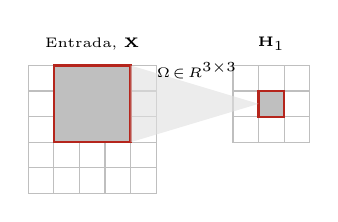
\begin{tikzpicture}[every node/.style={font=\scriptsize}, scale=0.65]
            % Entrada 5x5 com janela 3x3 destacada
            \fill[black!25] (0.5,1.0) rectangle (2.0,2.5);
            \draw[step=0.5, gray!50] (0,0) grid (2.5,2.5);
            \draw[gray!50] (0,0) rectangle (2.5,2.5);
            \draw[thick, BrickRed] (0.5,1.0) rectangle (2.0,2.5);
            \node[font=\tiny, anchor=south] at (1.25,2.6) {Entrada, $\mathbf{X}$};
            % H1 (3x3) com uma celula ativa
            \fill[black!25] (4.5,1.5) rectangle (5.0,2.0);
            \draw[step=0.5, gray!50] (4.0,1.0) grid (5.5,2.5);
            \draw[gray!50] (4.0,1.0) rectangle (5.5,2.5);
            \draw[thick, BrickRed] (4.5,1.5) rectangle (5.0,2.0);
            \node[font=\tiny, anchor=south] at (4.75,2.6) {$\mathbf{H}_1$};
            % Cone conectando a janela 3x3 ao ponto ativo
            \fill[gray!25, opacity=0.6] (2.0,2.5) -- (2.0,1.0) -- (4.5,1.75) -- cycle;
            \node[font=\tiny] at (3.3,2.4) {$\Omega\!\in\!\mathbb{R}^{3\times 3}$};
        \end{tikzpicture}
    \end{column}
\end{columns}
\end{frame}

\begin{frame}[shrink=5]{Crescimento do Campo Receptivo}
\begin{columns}[T]
    \begin{column}{.45\linewidth}
        \begin{itemize}
            \item Empilhando convoluções sucessivas, o campo receptivo cresce camada a camada.
            \begin{itemize}
                \item Cada unidade de $\mathbf{H}_2$ enxerga uma janela $3\times 3$ de $\mathbf{H}_1$, que por sua vez vem de uma janela $5\times 5$ na entrada.
                \item Isso permite construir representações cada vez mais ``globais'' da imagem.
            \end{itemize}
            \item Um campo receptivo pequeno pode perder informações relevantes.
            \item Convoluções com \textit{stride} maior que 1 aceleram esse crescimento, ao custo de reduzir a resolução espacial.
        \end{itemize}
    \end{column}
    \begin{column}{.55\linewidth}
        \centering
        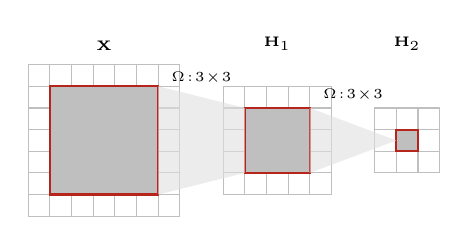
\begin{tikzpicture}[every node/.style={font=\scriptsize}, scale=0.55]
            % Entrada 7x7 com janela 5x5 ativa
            \fill[black!25] (0.5,0.5) rectangle (3.0,3.0);
            \draw[step=0.5, gray!50] (0,0) grid (3.5,3.5);
            \draw[gray!50] (0,0) rectangle (3.5,3.5);
            \draw[thick, BrickRed] (0.5,0.5) rectangle (3.0,3.0);
            \node[font=\tiny, anchor=south] at (1.75,3.6) {$\mathbf{X}$};
            % H1 5x5 com janela 3x3 ativa
            \fill[black!25] (5.0,1.0) rectangle (6.5,2.5);
            \draw[step=0.5, gray!50] (4.5,0.5) grid (7.0,3.0);
            \draw[gray!50] (4.5,0.5) rectangle (7.0,3.0);
            \draw[thick, BrickRed] (5.0,1.0) rectangle (6.5,2.5);
            \node[font=\tiny, anchor=south] at (5.75,3.6) {$\mathbf{H}_1$};
            % H2 3x3 com 1 celula ativa
            \fill[black!25] (8.5,1.5) rectangle (9.0,2.0);
            \draw[step=0.5, gray!50] (8.0,1.0) grid (9.5,2.5);
            \draw[gray!50] (8.0,1.0) rectangle (9.5,2.5);
            \draw[thick, BrickRed] (8.5,1.5) rectangle (9.0,2.0);
            \node[font=\tiny, anchor=south] at (8.75,3.6) {$\mathbf{H}_2$};
            % Cones
            \fill[gray!25, opacity=0.6] (3.0,3.0) -- (3.0,0.5) -- (5.0,1.0) -- (5.0,2.5) -- cycle;
            \fill[gray!25, opacity=0.6] (6.5,2.5) -- (6.5,1.0) -- (8.5,1.75) -- cycle;
            \node[font=\tiny] at (4.0,3.2) {$\Omega\!:\!3\!\times\!3$};
            \node[font=\tiny] at (7.5,2.8) {$\Omega\!:\!3\!\times\!3$};
        \end{tikzpicture}
    \end{column}
\end{columns}
\end{frame}

\begin{frame}{Fórmula do Campo Receptivo}
\begin{itemize}
    \item Para uma sequência de camadas com tamanho de kernel $K_l$ e \textit{stride} $S_l$, o campo receptivo $RF_l$ na camada $l$ obedece à recursão:
\end{itemize}
\begin{equation*}
    RF_l = RF_{l-1} + (K_l - 1) \prod_{i<l} S_i, \qquad RF_0 = 1.
\end{equation*}
\begin{itemize}
    \item Cada nova camada acrescenta $K_l - 1$ posições do espaço original, multiplicadas pelo produto acumulado dos \textit{strides} anteriores.
    \item \textbf{Exemplo}, três convoluções $3\times 3$ com $S=1$:
    \begin{itemize}
        \item $RF_1 = 1 + (3-1)\cdot 1 = 3$.
        \item $RF_2 = 3 + (3-1)\cdot 1 = 5$.
        \item $RF_3 = 5 + (3-1)\cdot 1 = 7$.
    \end{itemize}
    \item Se a segunda camada usa $S_2 = 2$, então $RF_3 = 3 + (3-1)\cdot 1 + (3-1)\cdot 2 = 9$, \textit{stride} acelera o crescimento do campo receptivo.
\end{itemize}
\end{frame}

% Grade n x n (celulas de 0.5) totalmente sombreada: #1 x-esq, #2 y-centro, #3 n
\newcommand{\rfgrade}[3]{%
    \pgfmathsetmacro{\rfh}{#3*0.5}%
    \pgfmathsetmacro{\rfylo}{#2-\rfh/2}%
    \pgfmathsetmacro{\rfyhi}{#2+\rfh/2}%
    \pgfmathsetmacro{\rfxhi}{#1+\rfh}%
    \fill[black!25] (#1,\rfylo) rectangle (\rfxhi,\rfyhi);
    \draw[gray!60, step=0.5, shift={(#1,\rfylo)}] (0,0) grid (\rfh,\rfh);
    \draw[thick, BrickRed] (#1,\rfylo) rectangle (\rfxhi,\rfyhi);
}
% Cone de conexao entre a borda direita de uma grade e a borda esquerda da proxima:
% #1 x-dir grade A, #2 y-centro, #3 n grade A, #4 x-esq grade B, #5 n grade B
\newcommand{\rfcone}[5]{%
    \pgfmathsetmacro{\rfha}{#3*0.25}%
    \pgfmathsetmacro{\rfhb}{#5*0.25}%
    \fill[gray!25, opacity=0.6] (#1,#2+\rfha) -- (#1,#2-\rfha) -- (#4,#2-\rfhb) -- (#4,#2+\rfhb) -- cycle;
}

\begin{frame}{Duas $3\times 3$ ou uma $5\times 5$?}
\begin{itemize}
    \item Duas convoluções $3\times 3$ sucessivas e uma única convolução $5\times 5$ produzem uma unidade com o mesmo campo receptivo: $5\times 5$ na entrada.
\end{itemize}
\centering
\begin{tikzpicture}[scale=0.7, every node/.style={font=\scriptsize}]
    % Opcao A: duas 3x3 (centro y=4.4)
    \node[anchor=east, align=right] at (-0.5,4.4) {\textbf{A}\\duas $3\times 3$};
    \rfcone{2.5}{4.4}{5}{4.0}{3}
    \rfcone{5.5}{4.4}{3}{7.0}{1}
    \rfgrade{0}{4.4}{5}
    \rfgrade{4.0}{4.4}{3}
    \rfgrade{7.0}{4.4}{1}
    \node[anchor=south] at (1.25,5.7) {$\mathbf{X}$};
    \node[anchor=south] at (4.75,5.2) {$\mathbf{H}_1$};
    \node[anchor=south] at (7.25,4.7) {$\mathbf{H}_2$};
    \node[anchor=north, font=\tiny] at (3.25,3.35) {\textit{kernel} $3\!\times\!3$};
    \node[anchor=north, font=\tiny] at (6.2,3.85) {\textit{kernel} $3\!\times\!3$};
    % Opcao B: uma 5x5 (centro y=1.0)
    \node[anchor=east, align=right] at (-0.5,1.0) {\textbf{B}\\uma $5\times 5$};
    \rfcone{2.5}{1.0}{5}{4.0}{1}
    \rfgrade{0}{1.0}{5}
    \rfgrade{4.0}{1.0}{1}
    \node[anchor=south] at (1.25,2.3) {$\mathbf{X}$};
    \node[anchor=south] at (4.25,1.3) {$\mathbf{H}_1$};
    \node[anchor=north, font=\tiny] at (3.25,0.2) {\textit{kernel} $5\!\times\!5$};
\end{tikzpicture}
\begin{block}{Pergunta}
    Qual das duas opções é preferível?
\end{block}
\end{frame}

\begin{frame}{Duas $3\times 3$ ou uma $5\times 5$?}
\begin{itemize}
    \item Resposta: \textbf{duas convoluções $3\times 3$}\footfullcite{simonyan2014vgg}.
    \begin{itemize}
        \item Menos parâmetros: $2 \cdot (3 \cdot 3) = 18$ pesos contra $5 \cdot 5 = 25$.
        \item Mais não linearidade: duas ativações em vez de uma.
    \end{itemize}
\end{itemize}
\vspace{0.3em}
\centering
\begin{tikzpicture}[scale=0.7, every node/.style={font=\scriptsize}]
    % Opcao A: duas 3x3 (centro y=4.4)
    \node[anchor=east, align=right] at (-0.5,4.4) {\textbf{A}\\duas $3\times 3$};
    \rfcone{2.5}{4.4}{5}{4.0}{3}
    \rfcone{5.5}{4.4}{3}{7.0}{1}
    \rfgrade{0}{4.4}{5}
    \rfgrade{4.0}{4.4}{3}
    \rfgrade{7.0}{4.4}{1}
    \node[anchor=south] at (1.25,5.7) {$\mathbf{X}$};
    \node[anchor=south] at (4.75,5.2) {$\mathbf{H}_1$};
    \node[anchor=south] at (7.25,4.7) {$\mathbf{H}_2$};
    \node[anchor=north, font=\tiny] at (3.25,3.35) {$3\!\times\!3 = 9$ pesos};
    \node[anchor=north, font=\tiny] at (6.2,3.85) {$3\!\times\!3 = 9$ pesos};
    \node[anchor=north, font=\tiny, ForestGreen] at (4.75,3.6) {ReLU};
    \node[anchor=north, font=\tiny, ForestGreen] at (7.25,4.1) {ReLU};
    \node[anchor=west, align=left] at (8.0,4.4) {$18$ pesos\\$2$ ativações};
    % Opcao B: uma 5x5 (centro y=1.0)
    \node[anchor=east, align=right] at (-0.5,1.0) {\textbf{B}\\uma $5\times 5$};
    \rfcone{2.5}{1.0}{5}{4.0}{1}
    \rfgrade{0}{1.0}{5}
    \rfgrade{4.0}{1.0}{1}
    \node[anchor=south] at (1.25,2.3) {$\mathbf{X}$};
    \node[anchor=south] at (4.25,1.3) {$\mathbf{H}_1$};
    \node[anchor=north, font=\tiny] at (3.25,0.2) {$5\!\times\!5 = 25$ pesos};
    \node[anchor=north, font=\tiny, ForestGreen] at (4.25,0.7) {ReLU};
    \node[anchor=west, align=left] at (8.0,1.0) {$25$ pesos\\$1$ ativação};
\end{tikzpicture}
\end{frame}

%========================================================================
\section{Treinamento}
%========================================================================

\begin{frame}{Treinamento}
\begin{itemize}
    \item \textit{Backprop} funciona naturalmente para convoluções.
    \begin{itemize}
        \item As derivadas parciais com relação a cada peso compartilhado precisam ser \textbf{acumuladas} (somadas) sobre todas as posições onde esse peso atua.
    \end{itemize}
\end{itemize}
\vspace{0.4em}
\begin{columns}
    \begin{column}{.55\linewidth}
        \footnotesize
        Para um \textit{kernel} $\mathbf{\Theta}$ de tamanho $2\times 2$ com pesos $w_{m,n}$, aplicado a uma entrada $\mathbf{X}$ para gerar a saída $\mathbf{Y}$, o gradiente da função de custo $\mathcal{L}$ com relação a cada peso é:
        \begin{align*}
            \frac{\partial \mathcal{L}}{\partial w_{1,1}} &= \sum_{i,j} x_{i,j}\,\frac{\partial \mathcal{L}}{\partial y_{i,j}}\\
            \frac{\partial \mathcal{L}}{\partial w_{1,2}} &= \sum_{i,j} x_{i,j+1}\,\frac{\partial \mathcal{L}}{\partial y_{i,j}}\\
            \frac{\partial \mathcal{L}}{\partial w_{2,1}} &= \sum_{i,j} x_{i+1,j}\,\frac{\partial \mathcal{L}}{\partial y_{i,j}}\\
            \frac{\partial \mathcal{L}}{\partial w_{2,2}} &= \sum_{i,j} x_{i+1,j+1}\,\frac{\partial \mathcal{L}}{\partial y_{i,j}}
        \end{align*}
    \end{column}
    \begin{column}{.45\linewidth}
        \centering
        \begin{tikzpicture}[every node/.style={font=\small}]
            \node[circle, draw, minimum size=24pt] (conv) at (0,0) {CONV};
            \draw[->, thick] (-2.4,1.4) node[left]{$\mathbf{X}$} -- (conv);
            \draw[->, thick] (-2.4,0) node[left]{$\mathbf{\Theta}$} -- (conv);
            \draw[->, thick] (-2.4,-1.4) node[left]{$\mathbf{b}$} -- (conv);
            \draw[->, thick] (conv) -- (2.0,0) node[right]{$\mathbf{Y}$};
            \node[BrickRed, font=\scriptsize, anchor=south] at (-1.9,1.2) {$\dfrac{\partial \mathcal{L}}{\partial \mathbf{X}}$};
            \node[BrickRed, font=\scriptsize, anchor=north] at (-2.1,-0.05) {$\dfrac{\partial \mathcal{L}}{\partial \mathbf{\Theta}}$};
            \node[BrickRed, font=\scriptsize, anchor=north] at (-1.9,-1.2) {$\dfrac{\partial \mathcal{L}}{\partial \mathbf{b}}$};
            \node[BrickRed, font=\scriptsize, anchor=south] at (1.3,0.05) {$\dfrac{\partial \mathcal{L}}{\partial \mathbf{Y}}$};
        \end{tikzpicture}
    \end{column}
\end{columns}
\end{frame}

%========================================================================
\section{Downsampling e Upsampling}
%========================================================================

\begin{frame}{\textit{Downsampling}}
\begin{columns}[T]
    \begin{column}{.55\linewidth}
        \begin{itemize}
            \item Subamostrar espacialmente a imagem pode ter o efeito de aumentar o campo receptivo de uma unidade oculta.
            \item As principais formas de subamostragem em CNN são:
            \begin{enumerate}
                \item Usar \textit{stride} maior que 1 na convolução.
                \item \textit{Max pooling}: mantém apenas o maior valor de cada janela.
                \item \textit{Average pooling}: usa a média dos valores de cada janela.
            \end{enumerate}
        \end{itemize}
    \end{column}
    \begin{column}{.45\linewidth}
        \centering
        \begin{tikzpicture}[every node/.style={font=\scriptsize}, scale=0.42]
            % --- Max pooling ---
            \fill[PastelBlue2!40] (0,2) rectangle (2,4);
            \fill[orange!30]      (2,2) rectangle (4,4);
            \fill[green!25]       (0,0) rectangle (2,2);
            \fill[BrickRed!25]    (2,0) rectangle (4,2);
            \draw[gray!60] (0,0) rectangle (4,4);
            \draw[gray!60] (1,0) -- (1,4);
            \draw[gray!60] (2,0) -- (2,4);
            \draw[gray!60] (3,0) -- (3,4);
            \draw[gray!60] (0,1) -- (4,1);
            \draw[gray!60] (0,2) -- (4,2);
            \draw[gray!60] (0,3) -- (4,3);
            \draw[thick, PastelBlue2!70!black] (0,2) rectangle (2,4);
            \draw[thick, orange!70!black]      (2,2) rectangle (4,4);
            \draw[thick, green!50!black]       (0,0) rectangle (2,2);
            \draw[thick, BrickRed!80]          (2,0) rectangle (4,2);
            \node at (0.5,3.5) {$1$};   \node at (1.5,3.5) {$3$};
            \node at (0.5,2.5) {$2$};   \node at (1.5,2.5) {$\mathbf{8}$};
            \node at (2.5,3.5) {$\mathbf{9}$};   \node at (3.5,3.5) {$4$};
            \node at (2.5,2.5) {$1$};   \node at (3.5,2.5) {$5$};
            \node at (0.5,1.5) {$4$};   \node at (1.5,1.5) {$2$};
            \node at (0.5,0.5) {$\mathbf{7}$};   \node at (1.5,0.5) {$1$};
            \node at (2.5,1.5) {$3$};   \node at (3.5,1.5) {$\mathbf{6}$};
            \node at (2.5,0.5) {$2$};   \node at (3.5,0.5) {$5$};
            \node[font=\tiny, anchor=south] at (2,4.05) {entrada};
            \draw[->, gray!70, thick] (4.2,2) -- (5.4,2);
            \node[font=\tiny, anchor=south] at (4.8,2.1) {max};
            \fill[PastelBlue2!40] (5.7,3) rectangle (6.7,4);
            \fill[orange!30]      (6.7,3) rectangle (7.7,4);
            \fill[green!25]       (5.7,2) rectangle (6.7,3);
            \fill[BrickRed!25]    (6.7,2) rectangle (7.7,3);
            \draw[gray!60] (5.7,2) rectangle (7.7,4);
            \draw[gray!60] (6.7,2) -- (6.7,4);
            \draw[gray!60] (5.7,3) -- (7.7,3);
            \node at (6.2,3.5) {$8$};
            \node at (7.2,3.5) {$9$};
            \node at (6.2,2.5) {$7$};
            \node at (7.2,2.5) {$6$};
            \node[font=\tiny, anchor=south] at (6.7,4.05) {saída};

            % --- Average pooling, deslocado para baixo ---
            \begin{scope}[yshift=-5cm]
            \fill[PastelBlue2!40] (0,2) rectangle (2,4);
            \fill[orange!30]      (2,2) rectangle (4,4);
            \fill[green!25]       (0,0) rectangle (2,2);
            \fill[BrickRed!25]    (2,0) rectangle (4,2);
            \draw[gray!60] (0,0) rectangle (4,4);
            \draw[gray!60] (1,0) -- (1,4);
            \draw[gray!60] (2,0) -- (2,4);
            \draw[gray!60] (3,0) -- (3,4);
            \draw[gray!60] (0,1) -- (4,1);
            \draw[gray!60] (0,2) -- (4,2);
            \draw[gray!60] (0,3) -- (4,3);
            \draw[thick, PastelBlue2!70!black] (0,2) rectangle (2,4);
            \draw[thick, orange!70!black]      (2,2) rectangle (4,4);
            \draw[thick, green!50!black]       (0,0) rectangle (2,2);
            \draw[thick, BrickRed!80]          (2,0) rectangle (4,2);
            \node at (0.5,3.5) {$2$};   \node at (1.5,3.5) {$4$};
            \node at (0.5,2.5) {$0$};   \node at (1.5,2.5) {$2$};
            \node at (2.5,3.5) {$6$};   \node at (3.5,3.5) {$8$};
            \node at (2.5,2.5) {$4$};   \node at (3.5,2.5) {$6$};
            \node at (0.5,1.5) {$1$};   \node at (1.5,1.5) {$3$};
            \node at (0.5,0.5) {$3$};   \node at (1.5,0.5) {$5$};
            \node at (2.5,1.5) {$5$};   \node at (3.5,1.5) {$7$};
            \node at (2.5,0.5) {$7$};   \node at (3.5,0.5) {$9$};
            \node[font=\tiny, anchor=south] at (2,4.05) {entrada};
            \draw[->, gray!70, thick] (4.2,2) -- (5.4,2);
            \node[font=\tiny, anchor=south] at (4.8,2.1) {avg};
            \fill[PastelBlue2!40] (5.7,3) rectangle (6.7,4);
            \fill[orange!30]      (6.7,3) rectangle (7.7,4);
            \fill[green!25]       (5.7,2) rectangle (6.7,3);
            \fill[BrickRed!25]    (6.7,2) rectangle (7.7,3);
            \draw[gray!60] (5.7,2) rectangle (7.7,4);
            \draw[gray!60] (6.7,2) -- (6.7,4);
            \draw[gray!60] (5.7,3) -- (7.7,3);
            \node at (6.2,3.5) {$2$};
            \node at (7.2,3.5) {$6$};
            \node at (6.2,2.5) {$3$};
            \node at (7.2,2.5) {$7$};
            \node[font=\tiny, anchor=south] at (6.7,4.05) {saída};
            \end{scope}
        \end{tikzpicture}
    \end{column}
\end{columns}
\end{frame}

\begin{frame}{\textit{Upsampling}}
\begin{columns}[T]
    \begin{column}{.55\linewidth}
        \begin{itemize}
            \item Sobreamostrar espacialmente pode ser útil quando a saída da rede também é uma imagem (segmentação, super resolução, geração).
            \item As principais formas de sobreamostragem em CNN são:
            \begin{enumerate}
                \item Duplicar os valores conhecidos.
                \item \textit{Max unpooling}: insere o valor na posição original do \textit{max pooling} e zera as demais.
                \item Interpolação bilinear.
                \item Convolução transposta.
            \end{enumerate}
        \end{itemize}
    \end{column}
    \begin{column}{.45\linewidth}
        \centering
        \begin{tikzpicture}[every node/.style={font=\scriptsize}, scale=0.42]
            % --- Duplicação de valores (nearest neighbor) ---
            \fill[PastelBlue2!40] (0,2) rectangle (1,3);
            \fill[orange!30]      (1,2) rectangle (2,3);
            \fill[green!25]       (0,1) rectangle (1,2);
            \fill[BrickRed!25]    (1,1) rectangle (2,2);
            \draw[gray!60] (0,1) rectangle (2,3);
            \draw[gray!60] (1,1) -- (1,3);
            \draw[gray!60] (0,2) -- (2,2);
            \node at (0.5,2.5) {$8$};
            \node at (1.5,2.5) {$9$};
            \node at (0.5,1.5) {$7$};
            \node at (1.5,1.5) {$6$};
            \node[font=\tiny, anchor=south] at (1,3.05) {entrada};
            \draw[->, gray!70, thick] (2.2,2) -- (5.2,2);
            \node[font=\tiny, anchor=south] at (3.7,2.1) {duplicar};
            \fill[PastelBlue2!40] (5.5,2) rectangle (7.5,4);
            \fill[orange!30]      (7.5,2) rectangle (9.5,4);
            \fill[green!25]       (5.5,0) rectangle (7.5,2);
            \fill[BrickRed!25]    (7.5,0) rectangle (9.5,2);
            \draw[gray!60] (5.5,0) rectangle (9.5,4);
            \draw[gray!60] (6.5,0) -- (6.5,4);
            \draw[gray!60] (7.5,0) -- (7.5,4);
            \draw[gray!60] (8.5,0) -- (8.5,4);
            \draw[gray!60] (5.5,1) -- (9.5,1);
            \draw[gray!60] (5.5,2) -- (9.5,2);
            \draw[gray!60] (5.5,3) -- (9.5,3);
            \node at (6.0,3.5) {$8$}; \node at (7.0,3.5) {$8$};
            \node at (8.0,3.5) {$9$}; \node at (9.0,3.5) {$9$};
            \node at (6.0,2.5) {$8$}; \node at (7.0,2.5) {$8$};
            \node at (8.0,2.5) {$9$}; \node at (9.0,2.5) {$9$};
            \node at (6.0,1.5) {$7$}; \node at (7.0,1.5) {$7$};
            \node at (8.0,1.5) {$6$}; \node at (9.0,1.5) {$6$};
            \node at (6.0,0.5) {$7$}; \node at (7.0,0.5) {$7$};
            \node at (8.0,0.5) {$6$}; \node at (9.0,0.5) {$6$};
            \node[font=\tiny, anchor=south] at (7.5,4.05) {saída};

            % --- Interpolação bilinear, deslocada para baixo ---
            \begin{scope}[yshift=-5cm]
            % Entrada 2x2
            \fill[PastelBlue2!40] (0,2) rectangle (1,3);
            \fill[orange!30]      (1,2) rectangle (2,3);
            \fill[green!25]       (0,1) rectangle (1,2);
            \fill[BrickRed!25]    (1,1) rectangle (2,2);
            \draw[gray!60] (0,1) rectangle (2,3);
            \draw[gray!60] (1,1) -- (1,3);
            \draw[gray!60] (0,2) -- (2,2);
            \node at (0.5,2.5) {$0$};
            \node at (1.5,2.5) {$3$};
            \node at (0.5,1.5) {$6$};
            \node at (1.5,1.5) {$9$};
            \node[font=\tiny, anchor=south] at (1,3.05) {entrada};
            \draw[->, gray!70, thick] (2.2,2) -- (5.2,2);
            \node[font=\tiny, anchor=south] at (3.7,2.1) {bilinear};
            % Saída 4x4 (valores interpolados, cantos mantêm os 4 originais)
            \fill[PastelBlue2!40] (5.5,2) rectangle (7.5,4);
            \fill[orange!30]      (7.5,2) rectangle (9.5,4);
            \fill[green!25]       (5.5,0) rectangle (7.5,2);
            \fill[BrickRed!25]    (7.5,0) rectangle (9.5,2);
            \draw[gray!60] (5.5,0) rectangle (9.5,4);
            \draw[gray!60] (6.5,0) -- (6.5,4);
            \draw[gray!60] (7.5,0) -- (7.5,4);
            \draw[gray!60] (8.5,0) -- (8.5,4);
            \draw[gray!60] (5.5,1) -- (9.5,1);
            \draw[gray!60] (5.5,2) -- (9.5,2);
            \draw[gray!60] (5.5,3) -- (9.5,3);
            \node at (6.0,3.5) {$0$}; \node at (7.0,3.5) {$1$};
            \node at (8.0,3.5) {$2$}; \node at (9.0,3.5) {$3$};
            \node at (6.0,2.5) {$2$}; \node at (7.0,2.5) {$3$};
            \node at (8.0,2.5) {$4$}; \node at (9.0,2.5) {$5$};
            \node at (6.0,1.5) {$4$}; \node at (7.0,1.5) {$5$};
            \node at (8.0,1.5) {$6$}; \node at (9.0,1.5) {$7$};
            \node at (6.0,0.5) {$6$}; \node at (7.0,0.5) {$7$};
            \node at (8.0,0.5) {$8$}; \node at (9.0,0.5) {$9$};
            \node[font=\tiny, anchor=south] at (7.5,4.05) {saída};
            \end{scope}
        \end{tikzpicture}
    \end{column}
\end{columns}
\end{frame}

\begin{frame}{Convolução Transposta}
\begin{itemize}
    \item Operação aprendível para aumentar a resolução espacial.
    \item Cada elemento da entrada multiplica o \textit{kernel} inteiro e o resultado é depositado em uma região da saída, com sobreposições somadas.
    \item Parâmetros: \textit{kernel size}, \textit{padding}, \textit{stride}. \textit{Stride} maior que 1 \textbf{expande} a saída.
\end{itemize}
\end{frame}

\begin{frame}{Convolução Transposta: Dois \textit{Paddings}}
\begin{columns}[T]
    \begin{column}{.5\linewidth}
        \begin{itemize}
            \item \textit{padding} $p$: recorta $p$ linhas e colunas de cada lado da saída completa.
            \item \textit{output\_padding}: acrescenta linhas e colunas na base e à direita.
            \item Na convolução direta, $\lfloor (n+2p-k)/s \rfloor + 1$ arredonda para baixo: entradas $3\times 3$ e $4\times 4$ geram a mesma saída $2\times 2$.
            \item O \textit{output\_padding} escolhe para qual tamanho a transposta volta.
        \end{itemize}
    \end{column}
    \begin{column}{.5\linewidth}
        \centering
        % Celulas de 0.33cm. Entradas com padding p=1 (borda tracejada); contorno roxo = area
        % alcancada pelas janelas 3x3 com stride 2 (indices com padding 0..4); em laranja, a primeira
        % janela 3x3 e a celula da saida que ela produz.
        \begin{tikzpicture}[every node/.style={font=\tiny}, x=0.33cm, y=0.33cm]
            % ---------- Linha de cima: n = 3 ----------
            \begin{scope}[shift={(0,7.5)}]
                \draw[step=1, gray!45, dashed] (0,0) grid (5,5);
                \draw[gray!45, dashed] (0,0) rectangle (5,5);
                \fill[PastelBlue2!35] (1,1) rectangle (4,4);
                \draw[step=1, gray!60] (1,1) grid (4,4);
                \draw[gray!60] (1,1) rectangle (4,4);
                \draw[thick, purple] (0,0) rectangle (5,5);
                \draw[very thick, orange!80!black] (0.12,2.12) rectangle (2.88,4.88);
                \node[anchor=south] at (2.5,5.1) {entrada $3\!\times\!3$, $p=1$};
            \end{scope}
            \draw[->, gray!70, thick] (6.0,10.0) -- node[above] {conv.} node[below, align=center] {$k=3$\\$s=2$} (9.0,10.0);
            \begin{scope}[shift={(9.5,9.0)}]
                \fill[orange!30] (0,0) rectangle (2,2);
                \draw[step=1, gray!60] (0,0) grid (2,2);
                \draw[gray!60] (0,0) rectangle (2,2);
                \draw[very thick, orange!80!black] (0.08,1.08) rectangle (0.92,1.92);
                \node[anchor=north] at (1,-0.1) {$2\!\times\!2$};
            \end{scope}
            \draw[->, gray!70, thick] (12.0,10.0) -- node[above] {transp.} node[below, align=center] {$k=3$\\$s=2$} (15.0,10.0);
            \begin{scope}[shift={(15.5,8.5)}]
                \fill[PastelBlue2!35] (0,0) rectangle (3,3);
                \draw[step=1, gray!60] (0,0) grid (3,3);
                \draw[gray!60] (0,0) rectangle (3,3);
                \node[anchor=north, align=center] at (1.5,-0.1) {$3\!\times\!3$\\\textit{output\_padding} $=0$};
            \end{scope}

            % ---------- Linha de baixo: n = 4 ----------
            \begin{scope}[shift={(0,0)}]
                \draw[step=1, gray!45, dashed] (0,0) grid (6,6);
                \draw[gray!45, dashed] (0,0) rectangle (6,6);
                \fill[PastelBlue2!35] (1,1) rectangle (5,5);
                \draw[step=1, gray!60] (1,1) grid (5,5);
                \draw[gray!60] (1,1) rectangle (5,5);
                \draw[thick, purple] (0,1) rectangle (5,6);
                \draw[very thick, orange!80!black] (0.12,3.12) rectangle (2.88,5.88);
                \node[anchor=north, align=center] at (3,-0.1) {entrada $4\!\times\!4$, $p=1$\\última linha e coluna\\fora das janelas};
            \end{scope}
            \draw[->, gray!70, thick] (6.5,3.0) -- node[above] {conv.} node[below, align=center] {$k=3$\\$s=2$} (9.0,3.0);
            \begin{scope}[shift={(9.5,2.0)}]
                \fill[orange!30] (0,0) rectangle (2,2);
                \draw[step=1, gray!60] (0,0) grid (2,2);
                \draw[gray!60] (0,0) rectangle (2,2);
                \draw[very thick, orange!80!black] (0.08,1.08) rectangle (0.92,1.92);
                \node[anchor=north] at (1,-0.1) {$2\!\times\!2$};
            \end{scope}
            \draw[->, gray!70, thick] (12.0,3.0) -- node[above] {transp.} node[below, align=center] {$k=3$\\$s=2$} (15.0,3.0);
            \begin{scope}[shift={(15.5,1.0)}]
                \fill[PastelBlue2!35] (0,1) rectangle (3,4);
                \fill[teal!15] (0,0) rectangle (4,1);
                \fill[teal!15] (3,1) rectangle (4,4);
                \draw[step=1, gray!60] (0,0) grid (4,4);
                \draw[gray!60] (0,0) rectangle (4,4);
                \draw[thick, teal!70!black, dashed] (0,0) -- (4,0) -- (4,4) -- (3,4) -- (3,1) -- (0,1) -- cycle;
                \node[anchor=north, align=center] at (2,-0.1) {$4\!\times\!4$\\\textit{output\_padding} $=1$};
            \end{scope}
        \end{tikzpicture}
    \end{column}
\end{columns}
\end{frame}

\begin{frame}{Convolução Transposta: Exemplo}
\begin{itemize}
    \item Filtro $3\times 3$, \textit{stride} $=2$, \textit{padding} $=1$, \textit{output\_padding} $=1$. Cada célula da entrada projeta o \textit{kernel} inteiro multiplicado por seu valor; sobreposições são somadas.
    \item Saída completa $5\times 5$: o \textit{padding} recorta a borda inteira e o \textit{output\_padding} devolve a última linha e a última coluna.
\end{itemize}
\vspace{0.2em}
\centering
\begin{tikzpicture}[every node/.style={font=\scriptsize}, scale=0.62,
    cory/.style={fill=orange!40},
    cpbb/.style={fill=PastelBlue2!45},
    cgrb/.style={fill=green!35},
    cbrb/.style={fill=BrickRed!35},
    tory/.style={text=orange!70!black},
    tpbb/.style={text=PastelBlue2!60!black},
    tgrb/.style={text=green!45!black},
    tbrb/.style={text=BrickRed},
    every cellnode/.style={font=\footnotesize}
]
    % Entrada 2x2
    \fill[cory] (0,1) rectangle (1,2);
    \fill[cpbb] (1,1) rectangle (2,2);
    \fill[cgrb] (0,0) rectangle (1,1);
    \fill[cbrb] (1,0) rectangle (2,1);
    \draw[step=1.0, gray!60] (0,0) grid (2,2);
    \draw[gray!60] (0,0) rectangle (2,2);
    \node at (0.5,1.5) {$2$}; \node at (1.5,1.5) {$1$};
    \node at (0.5,0.5) {$3$}; \node at (1.5,0.5) {$2$};
    \node[font=\tiny, anchor=south] at (1,2.05) {entrada $\mathbf{X}$};
    \only<2>{\draw[ultra thick, purple] (0,1) rectangle (1,2);}
    \only<3>{\draw[ultra thick, purple] (1,1) rectangle (2,2);}
    \only<4>{\draw[ultra thick, purple] (0,0) rectangle (1,1);}
    \only<5>{\draw[ultra thick, purple] (1,0) rectangle (2,1);}

    % Kernel 3x3
    \fill[PastelBlue2!15] (3.0,-0.5) rectangle (6.0,2.5);
    \draw[gray!60] (3.0,-0.5) rectangle (6.0,2.5);
    \draw[gray!60] (4.0,-0.5) -- (4.0,2.5);
    \draw[gray!60] (5.0,-0.5) -- (5.0,2.5);
    \draw[gray!60] (3.0,0.5) -- (6.0,0.5);
    \draw[gray!60] (3.0,1.5) -- (6.0,1.5);
    \node at (3.5,2.0) {$1$}; \node at (4.5,2.0) {$2$}; \node at (5.5,2.0) {$1$};
    \node at (3.5,1.0) {$2$}; \node at (4.5,1.0) {$0$}; \node at (5.5,1.0) {$1$};
    \node at (3.5,0.0) {$0$}; \node at (4.5,0.0) {$2$}; \node at (5.5,0.0) {$1$};
    \node[font=\tiny, anchor=south] at (4.5,2.55) {kernel $\mathbf{\Theta}$};

    % Saida completa 5x5 em escala maior para legibilidade (coordenadas locais: resultado 4x4
    % de (0,0) a (4,4); saida completa de (-1,0) a (4,5)). A borda inteira e recortada pelo
    % padding; a faixa em L (base e direita do resultado) e devolvida pelo output_padding.
    \begin{scope}[shift={(8.6,-2.0)}, xscale=1.6, yscale=1.2]
    \fill[gray!18] (-1,0) rectangle (4,5);
    \fill[white] (0,1) rectangle (3,4);
    \fill[teal!15] (0,0) rectangle (4,1);
    \fill[teal!15] (3,1) rectangle (4,4);
    \draw[step=1.0, gray!45, dashed] (-1,0) grid (4,5);
    \draw[gray!45, dashed] (-1,0) rectangle (4,5);
    \draw[step=1.0, gray!60] (0,0) grid (4,4);
    \draw[gray!60] (0,0) rectangle (4,4);
    \draw[thick, teal!70!black, dashed] (0,0) -- (4,0) -- (4,4) -- (3,4) -- (3,1) -- (0,1) -- cycle;
    \draw[thick, gray!70!black] (0,0) rectangle (4,4);
    \node[font=\tiny, anchor=south] at (1.5,5.05) {saída completa $5\!\times\!5$};

    % Regiao alcancada pelo kernel projetado da celula atual (3x3, inclui a borda recortada)
    \only<2>{\draw[ultra thick, purple] (-1,2) rectangle (2,5);}
    \only<3>{\draw[ultra thick, purple] (1,2) rectangle (4,5);}
    \only<4>{\draw[ultra thick, purple] (-1,0) rectangle (2,3);}
    \only<5>{\draw[ultra thick, purple] (1,0) rectangle (4,3);}

    % --- Borda recortada e nao devolvida (cores atenuadas) ---
    % Linha de cima (y=4.5)
    \node[font=\scriptsize] at (-0.5,4.5) {\only<2->{\textcolor{orange!70!black!45}{$2$}}};
    \node[font=\scriptsize] at (0.5,4.5) {\only<2->{\textcolor{orange!70!black!45}{$4$}}};
    \node[font=\scriptsize] at (1.5,4.5) {\only<2->{\textcolor{orange!70!black!45}{$2$}}\only<3->{\textcolor{PastelBlue2!60!black!45}{$+1$}}};
    \node[font=\scriptsize] at (2.5,4.5) {\only<3->{\textcolor{PastelBlue2!60!black!45}{$2$}}};
    \node[font=\scriptsize] at (3.5,4.5) {\only<3->{\textcolor{PastelBlue2!60!black!45}{$1$}}};
    % Coluna da esquerda (x=-0.5)
    \node[font=\scriptsize] at (-0.5,3.5) {\only<2->{\textcolor{orange!70!black!45}{$4$}}};
    \node[font=\scriptsize] at (-0.5,2.5) {\only<2->{\textcolor{orange!70!black!45}{$0$}}\only<4->{\textcolor{green!45!black!45}{$+3$}}};
    \node[font=\scriptsize] at (-0.5,1.5) {\only<4->{\textcolor{green!45!black!45}{$6$}}};
    \node[font=\scriptsize] at (-0.5,0.5) {\only<4->{\textcolor{green!45!black!45}{$0$}}};

    % --- Conteudo das celulas (um node por celula, conteudo cumulativo) ---
    % Cada celula compoe contribuicoes de input cells em ordem: yellow, blue, green, red
    % Row 1 (top, y=3.5)
    \node[font=\scriptsize] at (0.5,3.5) {\only<2->{\textcolor{orange!70!black}{$0$}}};
    \node[font=\scriptsize] at (1.5,3.5) {\only<2->{\textcolor{orange!70!black}{$2$}}\only<3->{\textcolor{PastelBlue2!60!black}{$+2$}}};
    \node[font=\scriptsize] at (2.5,3.5) {\only<3->{\textcolor{PastelBlue2!60!black}{$0$}}};
    \node[font=\scriptsize] at (3.5,3.5) {\only<3->{\textcolor{PastelBlue2!60!black}{$1$}}};
    % Row 2 (y=2.5)
    \node[font=\scriptsize] at (0.5,2.5) {\only<2->{\textcolor{orange!70!black}{$4$}}\only<4->{\textcolor{green!45!black}{$+6$}}};
    \node[font=\tiny] at (1.5,2.5) {\only<2->{\textcolor{orange!70!black}{$2$}}\only<3->{\textcolor{PastelBlue2!60!black}{${+}0$}}\only<4->{\textcolor{green!45!black}{${+}3$}}\only<5->{\textcolor{BrickRed}{${+}2$}}};
    \node[font=\scriptsize] at (2.5,2.5) {\only<3->{\textcolor{PastelBlue2!60!black}{$2$}}\only<5->{\textcolor{BrickRed}{$+4$}}};
    \node[font=\scriptsize] at (3.5,2.5) {\only<3->{\textcolor{PastelBlue2!60!black}{$1$}}\only<5->{\textcolor{BrickRed}{$+2$}}};
    % Row 3 (y=1.5)
    \node[font=\scriptsize] at (0.5,1.5) {\only<4->{\textcolor{green!45!black}{$0$}}};
    \node[font=\scriptsize] at (1.5,1.5) {\only<4->{\textcolor{green!45!black}{$3$}}\only<5->{\textcolor{BrickRed}{$+4$}}};
    \node[font=\scriptsize] at (2.5,1.5) {\only<5->{\textcolor{BrickRed}{$0$}}};
    \node[font=\scriptsize] at (3.5,1.5) {\only<5->{\textcolor{BrickRed}{$2$}}};
    % Row 4 (y=0.5)
    \node[font=\scriptsize] at (0.5,0.5) {\only<4->{\textcolor{green!45!black}{$6$}}};
    \node[font=\scriptsize] at (1.5,0.5) {\only<4->{\textcolor{green!45!black}{$3$}}\only<5->{\textcolor{BrickRed}{$+0$}}};
    \node[font=\scriptsize] at (2.5,0.5) {\only<5->{\textcolor{BrickRed}{$4$}}};
    \node[font=\scriptsize] at (3.5,0.5) {\only<5->{\textcolor{BrickRed}{$2$}}};
    \end{scope}

    % Legenda
    \begin{scope}[shift={(15.4,0.0)}, every node/.style={font=\tiny, anchor=west}]
    \fill[gray!18] (0,2.0) rectangle (0.5,2.4); \draw[gray!45, dashed] (0,2.0) rectangle (0.5,2.4);
    \node at (0.6,2.2) {recortado (\textit{padding})};
    \fill[teal!15] (0,1.2) rectangle (0.5,1.6); \draw[thick, teal!70!black, dashed] (0,1.2) rectangle (0.5,1.6);
    \node at (0.6,1.4) {devolvido (\textit{output\_padding})};
    \draw[thick, gray!70!black] (0,0.4) rectangle (0.5,0.8);
    \node at (0.6,0.6) {resultado $4\!\times\!4$};
    \end{scope}
\end{tikzpicture}
\end{frame}

\begin{frame}{Convolução $1\times 1$}
\begin{columns}[T]
    \begin{column}{.5\linewidth}
        \begin{itemize}
            \item Algumas vezes queremos mudar o número de canais sem agrupamento espacial.
            \begin{itemize}
                \item Nesses casos podemos aplicar a convolução $1\times 1$.
            \end{itemize}
            \item Cada posição espacial é independente: cada saída $h'_{i,j,c}$ é uma combinação linear dos canais de entrada $h_{i,j,1\dots C_i}$.
            \item Útil para reduzir ou expandir a profundidade do tensor sem alterar largura e altura.
        \end{itemize}
    \end{column}
    \begin{column}{.5\linewidth}
        \centering
        \begin{tikzpicture}[every node/.style={font=\scriptsize}, scale=0.5]
            % 3 canais de entrada empilhados (offset diagonal)
            \foreach \k/\clr/\dx/\dy in {3/PastelBlue2!15/0.5/0.5, 2/PastelBlue2!25/0.25/0.25, 1/PastelBlue2!40/0/0} {
                \fill[\clr] (\dx,\dy) rectangle (\dx+2.0,\dy+2.0);
                \draw[step=0.5, gray!50] (\dx,\dy) rectangle (\dx+2.0,\dy+2.0);
                \draw[gray!50] (\dx+0.5,\dy) -- (\dx+0.5,\dy+2.0);
                \draw[gray!50] (\dx+1.0,\dy) -- (\dx+1.0,\dy+2.0);
                \draw[gray!50] (\dx+1.5,\dy) -- (\dx+1.5,\dy+2.0);
                \draw[gray!50] (\dx,\dy+0.5) -- (\dx+2.0,\dy+0.5);
                \draw[gray!50] (\dx,\dy+1.0) -- (\dx+2.0,\dy+1.0);
                \draw[gray!50] (\dx,\dy+1.5) -- (\dx+2.0,\dy+1.5);
                \draw[thick, PastelBlue2!80!black] (\dx,\dy) rectangle (\dx+2.0,\dy+2.0);
            }
            \node[font=\tiny, anchor=south] at (1.25,3.0) {entrada (3 canais)};

            % Kernel 1x1 x 3 (coluna estreita de 3 celulas, cores empilhadas, centralizada no eixo do stack)
            \fill[BrickRed!45] (4.0,1.75) rectangle (4.5,2.25);
            \fill[BrickRed!30] (4.0,1.25) rectangle (4.5,1.75);
            \fill[BrickRed!15] (4.0,0.75) rectangle (4.5,1.25);
            \draw[gray!50] (4.0,0.75) rectangle (4.5,2.25);
            \draw[gray!50] (4.0,1.25) -- (4.5,1.25);
            \draw[gray!50] (4.0,1.75) -- (4.5,1.75);
            \draw[thick, BrickRed] (4.0,0.75) rectangle (4.5,2.25);
            \node[font=\tiny, anchor=north, align=center] at (4.25,0.70) {kernel\\$1\!\times\!1\!\times\!3$};

            % Canal de saida (1 canal)
            \fill[orange!25] (5.7,0.5) rectangle (7.7,2.5);
            \draw[step=0.5, gray!50, shift={(5.7,0.5)}] (0,0) grid (2.0,2.0);
            \draw[gray!50, shift={(5.7,0.5)}] (0,0) rectangle (2.0,2.0);
            \draw[thick, orange!70!black] (5.7,0.5) rectangle (7.7,2.5);
            \node[font=\tiny, anchor=south] at (6.7,2.55) {saída (1 canal)};

            % Setas
            \draw[->, gray!70, thick] (3.05,1.5) -- (3.95,1.5);
            \draw[->, gray!70, thick] (4.55,1.5) -- (5.65,1.5);
        \end{tikzpicture}
    \end{column}
\end{columns}
\end{frame}

%========================================================================
\section{Implementação de Convolução}
%========================================================================

\begin{frame}[fragile]{Implementação: Versão Ingênua}
\begin{itemize}
    \item Itera explicitamente por linhas, colunas, canais e \textit{kernel}:
\end{itemize}
\begin{lstlisting}[style=vscode-light, basicstyle=\ttfamily\scriptsize, language=Python]
# Versao com um unico canal de saida (C_o = 1).
# Para multiplos canais de saida bastaria envolver tudo
# em mais um loop sobre co e indexar feat_map_out[m, n, co].
for m in range(0, M):           # linhas
    for n in range(0, N):       # colunas
        for c in range(0, C):   # canais de entrada
            for i in range(0, K):     # tamanho kernel
                for j in range(0, K): # tamanho kernel
                    feat_map_out[m, n] += kernel[i, j, c] * feat_map_in[m+i, n+j, c]
        feat_map_out[m, n] += bias
\end{lstlisting}
\begin{itemize}
    \item Simples de entender, mas extremamente lenta e sem aproveitar paralelismo de hardware.
\end{itemize}
\end{frame}

\begin{frame}{Implementação: via Transformada de Fourier}
\begin{itemize}
    \item Versão complexa e raramente utilizada na prática.
    \item Convolução no domínio espacial é equivalente a multiplicação no domínio da frequência:
\end{itemize}
\begin{equation*}
    g(x) = f(x) * h(x) \qquad \Longleftrightarrow \qquad G(u) = F(u)\,H(u)
\end{equation*}
\vspace{-0.4em}
\begin{center}
\begin{tikzpicture}[every node/.style={font=\scriptsize},
    box/.style={draw, rounded corners=2pt, minimum width=1.6cm, minimum height=0.55cm, inner sep=1pt},
    sig/.style={draw, rounded corners=2pt, minimum width=0.9cm, minimum height=0.55cm, inner sep=1pt},
    op/.style={draw, circle, minimum size=0.45cm, inner sep=0pt},
    >=stealth
]
    \node[sig, fill=pink!50] (f) at (0,0.6) {$f(x)$};
    \node[sig, fill=yellow!40] (h) at (0,-0.6) {$h(x)$};
    \node[box, fill=gray!20] (ff) at (1.8,0.6) {FFT};
    \node[box, fill=gray!20] (fh) at (1.8,-0.6) {FFT};
    \node[sig, fill=pink!80] (F) at (3.6,0.6) {$F(u)$};
    \node[sig, fill=yellow!80] (H) at (3.6,-0.6) {$H(u)$};
    \node[op, fill=PastelBlue2!30] (mul) at (5.0,0) {$\times$};
    \node[box, fill=gray!20] (ifft) at (6.8,0) {IFFT};
    \node[sig, fill=green!40, minimum width=1.2cm] (out) at (8.6,0) {$f * h$};
    \draw[->] (f) -- (ff);
    \draw[->] (h) -- (fh);
    \draw[->] (ff) -- (F);
    \draw[->] (fh) -- (H);
    \draw[->] (F.east) -- (mul);
    \draw[->] (H.east) -- (mul);
    \draw[->] (mul) -- (ifft);
    \draw[->] (ifft) -- (out);
\end{tikzpicture}
\end{center}
\begin{itemize}
    \item Útil para convoluções com \textit{kernels} grandes (acima de $11\times 11$)\footfullcite{vasilache2014fbfft}.
\end{itemize}
\end{frame}

\begin{frame}{Implementação: \texttt{im2col} e Matriz de Toeplitz}
\begin{itemize}
    \item Versão utilizada na prática em GPUs e bibliotecas otimizadas.
    \item Existe uma forma inteligente de organizar a matriz de pesos para obter o resultado da convolução com uma única multiplicação de matrizes.
    \item Uma \textbf{matriz de Toeplitz} é uma matriz cujas diagonais principal e subdiagonais são constantes:
\end{itemize}
\begin{equation*}
\begin{bmatrix}
5 & 27 & 2 & -56 & 0 & 1 \\
-3 & 5 & 27 & 2 & -56 & 0 \\
8 & -3 & 5 & 27 & 2 & -56 \\
1 & 8 & -3 & 5 & 27 & 2 \\
-9 & 1 & 8 & -3 & 5 & 27 \\
3 & -9 & 1 & 8 & -3 & 5
\end{bmatrix}
\end{equation*}
\end{frame}

\begin{frame}{\texttt{im2col}: Passo 1 -- Entrada e filtro}
\begin{itemize}
    \item Definimos a entrada $\mathbf{X}$ ($3\times 3$) e o filtro $\mathbf{\Theta}$ ($2\times 2$):
\end{itemize}
\vspace{0.4em}
\centering
\begin{tikzpicture}[every node/.style={font=\footnotesize}, scale=0.8]
    % X 3x3 azul
    \node at (-0.7,1.5) {$\mathbf{X} = $};
    \fill[PastelBlue2!35] (0,0) rectangle (3,3);
    \draw[step=1, gray!60] (0,0) grid (3,3);
    \draw[gray!60] (0,0) rectangle (3,3);
    \node at (0.5,2.5) {$x_{1,1}$}; \node at (1.5,2.5) {$x_{1,2}$}; \node at (2.5,2.5) {$x_{1,3}$};
    \node at (0.5,1.5) {$x_{2,1}$}; \node at (1.5,1.5) {$x_{2,2}$}; \node at (2.5,1.5) {$x_{2,3}$};
    \node at (0.5,0.5) {$x_{3,1}$}; \node at (1.5,0.5) {$x_{3,2}$}; \node at (2.5,0.5) {$x_{3,3}$};
    % w 2x2 laranja
    \node at (5.3,1.5) {$\mathbf{\Theta} = $};
    \fill[orange!40] (6.0,0.5) rectangle (8.0,2.5);
    \draw[gray!60] (6.0,0.5) rectangle (8.0,2.5);
    \draw[gray!60] (7.0,0.5) -- (7.0,2.5);
    \draw[gray!60] (6.0,1.5) -- (8.0,1.5);
    \node at (6.5,2.0) {$w_{1,1}$}; \node at (7.5,2.0) {$w_{1,2}$};
    \node at (6.5,1.0) {$w_{2,1}$}; \node at (7.5,1.0) {$w_{2,2}$};
\end{tikzpicture}
\end{frame}

\begin{frame}{\texttt{im2col}: Passo 2 -- Tamanho da saída}
\begin{itemize}
    \item O tamanho da saída depende das janelas consideradas. Para $\mathbf{X}$~($3\times 3$) e $\mathbf{\Theta}$~($2\times 2$):
\end{itemize}
\vspace{0.4em}
\centering
{\small
\begin{tabular}{llcc}
    \toprule
    Modo & Janelas consideradas & Tamanho da saída & Exemplo \\
    \midrule
    \rowcolor{orange!15}
    \textbf{full} & sobreposição de pelo menos um pixel & $(X_h + w_h - 1)\times(X_w + w_w - 1)$ & $\mathbf{4\times 4}$ \\
    \textbf{valid} & inteiramente dentro da entrada & $(X_h - w_h + 1)\times(X_w - w_w + 1)$ & $2\times 2$ \\
    \textbf{same} & com \textit{padding} para manter o tamanho & $X_h \times X_w$ & $3\times 3$ \\
    \bottomrule
\end{tabular}
}
\vspace{0.6em}
\begin{itemize}
    \item Nos próximos passos calculamos o modo \textbf{full} ($4\times 4$), que é o que a construção com matrizes de Toeplitz produz diretamente.
    \item O modo \textit{valid}, o mais comum em CNNs, corresponde às $2\times 2$ posições centrais da saída \textit{full}.
\end{itemize}
\end{frame}

\begin{frame}{\texttt{im2col}: Passo 3 -- Zero padding do filtro}
\begin{itemize}
    \item A construção com matrizes de Toeplitz calcula a convolução com o \textit{kernel} rotacionado em $180^\circ$. Para obter a correlação cruzada usada em CNNs, rotacionamos $\mathbf{\Theta}$ antes.
    \item Depois aplicamos \textit{zero padding} no filtro rotacionado até atingir o tamanho da saída $4\times 4$:
\end{itemize}
\vspace{0.4em}
\centering
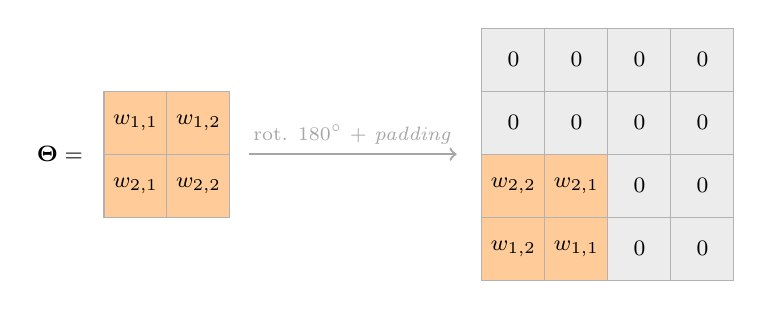
\begin{tikzpicture}[every node/.style={font=\footnotesize}, scale=0.8]
    % Theta original
    \node at (-1.9,2.0) {$\mathbf{\Theta} = $};
    \fill[orange!40] (-1.2,1.0) rectangle (0.8,3.0);
    \draw[step=1, gray!60, shift={(-1.2,1.0)}] (0,0) grid (2,2);
    \draw[gray!60, shift={(-1.2,1.0)}] (0,0) rectangle (2,2);
    \node at (-0.7,2.5) {$w_{1,1}$}; \node at (0.3,2.5) {$w_{1,2}$};
    \node at (-0.7,1.5) {$w_{2,1}$}; \node at (0.3,1.5) {$w_{2,2}$};
    \draw[->, gray!70, thick] (1.1,2.0) -- node[above, font=\scriptsize] {rot. $180^\circ$ + \textit{padding}} (4.4,2.0);
    % Padded 4x4: zeros no topo e a direita, pesos rotacionados no canto inferior-esquerdo
    \begin{scope}[shift={(4.8,0)}]
    \fill[gray!15] (0,0) rectangle (4,4);
    \fill[orange!40] (0,0) rectangle (2,2);
    \draw[step=1, gray!60] (0,0) grid (4,4);
    \draw[gray!60] (0,0) rectangle (4,4);
    \node at (0.5,3.5) {$0$}; \node at (1.5,3.5) {$0$}; \node at (2.5,3.5) {$0$}; \node at (3.5,3.5) {$0$};
    \node at (0.5,2.5) {$0$}; \node at (1.5,2.5) {$0$}; \node at (2.5,2.5) {$0$}; \node at (3.5,2.5) {$0$};
    \node at (0.5,1.5) {$w_{2,2}$}; \node at (1.5,1.5) {$w_{2,1}$};
    \node at (2.5,1.5) {$0$};       \node at (3.5,1.5) {$0$};
    \node at (0.5,0.5) {$w_{1,2}$}; \node at (1.5,0.5) {$w_{1,1}$};
    \node at (2.5,0.5) {$0$};       \node at (3.5,0.5) {$0$};
    \end{scope}
\end{tikzpicture}
\end{frame}

\begin{frame}{\texttt{im2col}: Passo 4 -- Matrizes de Toeplitz por linha}
\begin{itemize}
    \item Para cada linha do filtro paddado, construímos uma matriz de Toeplitz $\mathbf{F}_k$ (tamanho saída$_h \times$ entrada$_w = 4\times 3$). Começamos pela última linha.
\end{itemize}
\vspace{0.3em}
\centering
\begin{tikzpicture}[every node/.style={font=\tiny}, scale=0.55]
    % F0 azul (da linha 4 do padded: w_{1,2}, w_{1,1}, 0, 0)
    \node[anchor=south, font=\scriptsize] at (1.5,4.2) {$\mathbf{F}_0$};
    \fill[PastelBlue2!35] (0,0) rectangle (3,4);
    \draw[step=1, gray!60] (0,0) grid (3,4);
    \draw[gray!60] (0,0) rectangle (3,4);
    \node at (0.5,3.5) {$w_{1,2}$}; \node at (1.5,3.5) {$0$}; \node at (2.5,3.5) {$0$};
    \node at (0.5,2.5) {$w_{1,1}$}; \node at (1.5,2.5) {$w_{1,2}$}; \node at (2.5,2.5) {$0$};
    \node at (0.5,1.5) {$0$}; \node at (1.5,1.5) {$w_{1,1}$}; \node at (2.5,1.5) {$w_{1,2}$};
    \node at (0.5,0.5) {$0$}; \node at (1.5,0.5) {$0$}; \node at (2.5,0.5) {$w_{1,1}$};
    % F1 cinza (linha 3: w_{2,2}, w_{2,1}, 0, 0)
    \node[anchor=south, font=\scriptsize] at (5.5,4.2) {$\mathbf{F}_1$};
    \fill[black!15] (4,0) rectangle (7,4);
    \draw[step=1, gray!60] (4,0) grid (7,4);
    \draw[gray!60] (4,0) rectangle (7,4);
    \node at (4.5,3.5) {$w_{2,2}$}; \node at (5.5,3.5) {$0$}; \node at (6.5,3.5) {$0$};
    \node at (4.5,2.5) {$w_{2,1}$}; \node at (5.5,2.5) {$w_{2,2}$}; \node at (6.5,2.5) {$0$};
    \node at (4.5,1.5) {$0$}; \node at (5.5,1.5) {$w_{2,1}$}; \node at (6.5,1.5) {$w_{2,2}$};
    \node at (4.5,0.5) {$0$}; \node at (5.5,0.5) {$0$}; \node at (6.5,0.5) {$w_{2,1}$};
    % F2 laranja (linha 2: zeros)
    \node[anchor=south, font=\scriptsize] at (9.5,4.2) {$\mathbf{F}_2$};
    \fill[orange!30] (8,0) rectangle (11,4);
    \draw[step=1, gray!60] (8,0) grid (11,4);
    \draw[gray!60] (8,0) rectangle (11,4);
    \foreach \r in {0.5,1.5,2.5,3.5} \foreach \c in {8.5,9.5,10.5} \node at (\c,\r) {$0$};
    % F3 verde (linha 1: zeros)
    \node[anchor=south, font=\scriptsize] at (13.5,4.2) {$\mathbf{F}_3$};
    \fill[green!25] (12,0) rectangle (15,4);
    \draw[step=1, gray!60] (12,0) grid (15,4);
    \draw[gray!60] (12,0) rectangle (15,4);
    \foreach \r in {0.5,1.5,2.5,3.5} \foreach \c in {12.5,13.5,14.5} \node at (\c,\r) {$0$};
\end{tikzpicture}
\vspace{0.3em}
\begin{itemize}
    \item $\mathbf{F}_0$ vem da última linha do filtro paddado, $\mathbf{F}_1$ da penúltima, e assim por diante.
\end{itemize}
\end{frame}

\begin{frame}{\texttt{im2col}: Passo 5 -- Matriz de bloco Toeplitz}
\begin{itemize}
    \item Empilhamos as $F_k$ em uma matriz por blocos. O tamanho final é $16 \times 9$.
\end{itemize}
\vspace{0.4em}
\begin{columns}[T]
    \begin{column}{.45\linewidth}
        \centering
        \begin{equation*}
        \text{Bloco Toeplitz} =
        \begin{bmatrix}
        \textcolor{PastelBlue2!60!black}{\mathbf{F}_0} & 0 & 0 \\
        \textcolor{black!50}{\mathbf{F}_1} & \textcolor{PastelBlue2!60!black}{\mathbf{F}_0} & 0 \\
        \textcolor{orange!70!black}{\mathbf{F}_2} & \textcolor{black!50}{\mathbf{F}_1} & \textcolor{PastelBlue2!60!black}{\mathbf{F}_0} \\
        \textcolor{green!50!black}{\mathbf{F}_3} & \textcolor{orange!70!black}{\mathbf{F}_2} & \textcolor{black!50}{\mathbf{F}_1}
        \end{bmatrix}
        \end{equation*}
    \end{column}
    \begin{column}{.55\linewidth}
        \centering
        \begin{tikzpicture}[scale=0.28, every node/.style={font=\tiny}]
            % 16x9 grid: 4 block rows x 3 block cols, each block 4x3
            % Block (br, bc) at position (bc*3, (3-br)*4)
            % br=0 -> top, br=3 -> bottom
            % Top row: F_0, 0, 0
            \fill[PastelBlue2!35] (0,12) rectangle (3,16);
            \fill[gray!10] (3,12) rectangle (6,16);
            \fill[gray!10] (6,12) rectangle (9,16);
            % Second row: F_1, F_0, 0
            \fill[black!15] (0,8) rectangle (3,12);
            \fill[PastelBlue2!35] (3,8) rectangle (6,12);
            \fill[gray!10] (6,8) rectangle (9,12);
            % Third: F_2, F_1, F_0
            \fill[orange!30] (0,4) rectangle (3,8);
            \fill[black!15] (3,4) rectangle (6,8);
            \fill[PastelBlue2!35] (6,4) rectangle (9,8);
            % Bottom: F_3, F_2, F_1
            \fill[green!25] (0,0) rectangle (3,4);
            \fill[orange!30] (3,0) rectangle (6,4);
            \fill[black!15] (6,0) rectangle (9,4);
            \draw[step=1, gray!50] (0,0) grid (9,16);
            \draw[gray!50] (0,0) rectangle (9,16);
            \draw[very thick, gray!80] (0,0) rectangle (9,16);
            \draw[very thick, gray!80] (3,0) -- (3,16);
            \draw[very thick, gray!80] (6,0) -- (6,16);
            \draw[very thick, gray!80] (0,4) -- (9,4);
            \draw[very thick, gray!80] (0,8) -- (9,8);
            \draw[very thick, gray!80] (0,12) -- (9,12);
            \node[anchor=east] at (-0.3,8) {\scriptsize $16$};
            \node[anchor=north] at (4.5,-0.3) {\scriptsize $9$};
        \end{tikzpicture}
    \end{column}
\end{columns}
\vspace{0.3em}
\begin{itemize}
    \item Colunas $=$ linhas da imagem original ($3$); linhas $=$ linhas da imagem de saída vezes a largura ($4 \cdot 4 = 16$).
\end{itemize}
\end{frame}

\begin{frame}{\texttt{im2col}: Passo 6 -- Vetorização da entrada}
\begin{itemize}
    \item Vetorizamos $\mathbf{X}$ concatenando as linhas \textbf{de baixo para cima}:
\end{itemize}
\vspace{0.4em}
\centering
\begin{tikzpicture}[every node/.style={font=\footnotesize}, scale=0.7]
    % X 3x3 azul
    \node at (-0.7,1.5) {$\mathbf{X} = $};
    \fill[PastelBlue2!35] (0,0) rectangle (3,3);
    \draw[step=1, gray!60] (0,0) grid (3,3);
    \draw[gray!60] (0,0) rectangle (3,3);
    \node at (0.5,2.5) {$x_{1,1}$}; \node at (1.5,2.5) {$x_{1,2}$}; \node at (2.5,2.5) {$x_{1,3}$};
    \node at (0.5,1.5) {$x_{2,1}$}; \node at (1.5,1.5) {$x_{2,2}$}; \node at (2.5,1.5) {$x_{2,3}$};
    \node at (0.5,0.5) {$x_{3,1}$}; \node at (1.5,0.5) {$x_{3,2}$}; \node at (2.5,0.5) {$x_{3,3}$};
    % Arrow
    \draw[->, gray!70, thick] (3.4,1.5) -- (5.1,1.5);
    % Vector 9x1
    \fill[PastelBlue2!35] (5.5,-3.0) rectangle (6.5,6.0);
    \draw[gray!60] (5.5,-3.0) rectangle (6.5,6.0);
    \foreach \y in {-2,-1,0,1,2,3,4,5}{
        \draw[gray!60] (5.5,\y) -- (6.5,\y);
    }
    \node at (6.0,5.5) {$x_{3,1}$};
    \node at (6.0,4.5) {$x_{3,2}$};
    \node at (6.0,3.5) {$x_{3,3}$};
    \node at (6.0,2.5) {$x_{2,1}$};
    \node at (6.0,1.5) {$x_{2,2}$};
    \node at (6.0,0.5) {$x_{2,3}$};
    \node at (6.0,-0.5) {$x_{1,1}$};
    \node at (6.0,-1.5) {$x_{1,2}$};
    \node at (6.0,-2.5) {$x_{1,3}$};
\end{tikzpicture}
\end{frame}

\begin{frame}{\texttt{im2col}: Passo 7 -- Multiplicação e \textit{reshape}}
\begin{itemize}
    \item Multiplicamos a matriz de bloco Toeplitz pelo vetor de entrada e fazemos \textit{reshape} para a forma da saída:
\end{itemize}
\begin{equation*}
    \underbrace{\mathbf{T}}_{16 \times 9} \cdot \underbrace{\mathbf{x}}_{9 \times 1} = \underbrace{\mathbf{y}}_{16 \times 1}
    \;\;\xrightarrow{\;\text{reshape}\;}\;\;
    \underbrace{\mathbf{Y}}_{4 \times 4}
\end{equation*}
\begin{itemize}
    \item Cada linha do produto $\mathbf{T}\mathbf{x}$ já contém o resultado de uma posição da convolução; basta reorganizar em uma matriz $4\times 4$.
    \item O resultado é exatamente igual ao da convolução tradicional, calculado em \textbf{uma única multiplicação de matrizes}.
\end{itemize}
\end{frame}

\begin{frame}{\texttt{im2col}: Passo 8 -- Produto por blocos}
\begin{itemize}
    \item Separando $\mathbf{x}$ pelas linhas da imagem ($\mathbf{x}_3$, $\mathbf{x}_2$, $\mathbf{x}_1$), cada bloco de $\mathbf{y}$ é uma soma de produtos $\mathbf{F}_k\mathbf{x}_j$. Como $\mathbf{F}_2 = \mathbf{F}_3 = \mathbf{0}$, sobram poucos termos:
\end{itemize}
\vspace{0.6em}
\centering
\begin{tikzpicture}[every node/.style={font=\tiny}, scale=0.58]
    % ---------- Produto por blocos: T (4x3 blocos) . x (3 blocos) = y (4 blocos) ----------
    \fill[PastelBlue2!35] (0,3) rectangle (1,4); \node at (0.5,3.5) {$\mathbf{F}_0$};
    \fill[gray!10] (1,3) rectangle (2,4); \node at (1.5,3.5) {$0$};
    \fill[gray!10] (2,3) rectangle (3,4); \node at (2.5,3.5) {$0$};
    \fill[black!15] (0,2) rectangle (1,3); \node at (0.5,2.5) {$\mathbf{F}_1$};
    \fill[PastelBlue2!35] (1,2) rectangle (2,3); \node at (1.5,2.5) {$\mathbf{F}_0$};
    \fill[gray!10] (2,2) rectangle (3,3); \node at (2.5,2.5) {$0$};
    \fill[orange!30] (0,1) rectangle (1,2); \node at (0.5,1.5) {$\mathbf{F}_2$};
    \fill[black!15] (1,1) rectangle (2,2); \node at (1.5,1.5) {$\mathbf{F}_1$};
    \fill[PastelBlue2!35] (2,1) rectangle (3,2); \node at (2.5,1.5) {$\mathbf{F}_0$};
    \fill[green!25] (0,0) rectangle (1,1); \node at (0.5,0.5) {$\mathbf{F}_3$};
    \fill[orange!30] (1,0) rectangle (2,1); \node at (1.5,0.5) {$\mathbf{F}_2$};
    \fill[black!15] (2,0) rectangle (3,1); \node at (2.5,0.5) {$\mathbf{F}_1$};
    \draw[step=1, gray!60] (0,0) grid (3,4);
    \draw[gray!60] (0,0) rectangle (3,4);
    \draw[very thick, gray!80] (0,0) rectangle (3,4);
    \node[anchor=south, font=\scriptsize] at (1.5,4.1) {$\mathbf{T}$};
    \node[font=\footnotesize] at (3.5,2) {$\cdot$};
    % x em blocos (linhas de X, de baixo para cima)
    \fill[PastelBlue2!35] (4,0.5) rectangle (5,3.5);
    \draw[step=1, gray!60, shift={(0,0.5)}] (4,0) grid (5,3);
    \draw[gray!60, shift={(0,0.5)}] (4,0) rectangle (5,3);
    \node at (4.5,3.0) {$\mathbf{x}_3$}; \node at (4.5,2.0) {$\mathbf{x}_2$}; \node at (4.5,1.0) {$\mathbf{x}_1$};
    \node[anchor=south, font=\scriptsize] at (4.5,4.1) {$\mathbf{x}$};
    \node[font=\footnotesize] at (5.6,2) {$=$};
    % y em blocos
    \fill[yellow!30] (6.2,0) rectangle (9.2,4);
    \draw[gray!60] (6.2,0) rectangle (9.2,4);
    \foreach \y in {1,2,3} \draw[gray!60] (6.2,\y) -- (9.2,\y);
    \node at (7.7,3.5) {$\mathbf{F}_0\mathbf{x}_3$};
    \node at (7.7,2.5) {$\mathbf{F}_1\mathbf{x}_3 + \mathbf{F}_0\mathbf{x}_2$};
    \node at (7.7,1.5) {$\mathbf{F}_1\mathbf{x}_2 + \mathbf{F}_0\mathbf{x}_1$};
    \node at (7.7,0.5) {$\mathbf{F}_1\mathbf{x}_1$};
    \node[anchor=south, font=\scriptsize] at (7.7,4.1) {$\mathbf{y}$};
    \foreach \k/\y in {0/3.5,1/2.5,2/1.5,3/0.5} \node[anchor=west] at (9.25,\y) {$\mathbf{y}_\k$};

    % ---------- Exemplo: y_0 = F_0 x_3 elemento a elemento ----------
    \begin{scope}[shift={(11.9,0)}]
    \fill[PastelBlue2!35] (0,0) rectangle (3,4);
    \draw[step=1, gray!60] (0,0) grid (3,4);
    \draw[gray!60] (0,0) rectangle (3,4);
    \node at (0.5,3.5) {$w_{1,2}$}; \node at (1.5,3.5) {$0$}; \node at (2.5,3.5) {$0$};
    \node at (0.5,2.5) {$w_{1,1}$}; \node at (1.5,2.5) {$w_{1,2}$}; \node at (2.5,2.5) {$0$};
    \node at (0.5,1.5) {$0$}; \node at (1.5,1.5) {$w_{1,1}$}; \node at (2.5,1.5) {$w_{1,2}$};
    \node at (0.5,0.5) {$0$}; \node at (1.5,0.5) {$0$}; \node at (2.5,0.5) {$w_{1,1}$};
    \node[anchor=south, font=\scriptsize] at (1.5,4.1) {$\mathbf{F}_0$};
    \node[font=\footnotesize] at (3.5,2) {$\cdot$};
    \fill[PastelBlue2!35] (4,0.5) rectangle (5,3.5);
    \draw[step=1, gray!60, shift={(0,0.5)}] (4,0) grid (5,3);
    \draw[gray!60, shift={(0,0.5)}] (4,0) rectangle (5,3);
    \node at (4.5,3.0) {$x_{3,1}$}; \node at (4.5,2.0) {$x_{3,2}$}; \node at (4.5,1.0) {$x_{3,3}$};
    \node[anchor=south, font=\scriptsize] at (4.5,4.1) {$\mathbf{x}_3$};
    \node[font=\footnotesize] at (5.6,2) {$=$};
    \fill[yellow!30] (6.2,0) rectangle (10.2,4);
    \draw[gray!60] (6.2,0) rectangle (10.2,4);
    \foreach \y in {1,2,3} \draw[gray!60] (6.2,\y) -- (10.2,\y);
    \node at (8.2,3.5) {$w_{1,2}x_{3,1}$};
    \node at (8.2,2.5) {$w_{1,1}x_{3,1} + w_{1,2}x_{3,2}$};
    \node at (8.2,1.5) {$w_{1,1}x_{3,2} + w_{1,2}x_{3,3}$};
    \node at (8.2,0.5) {$w_{1,1}x_{3,3}$};
    \node[anchor=south, font=\scriptsize] at (8.2,4.1) {$\mathbf{y}_0$};
    \end{scope}
\end{tikzpicture}
\vspace{0.6em}
\begin{itemize}
    \item À direita, o bloco $\mathbf{y}_0$ calculado elemento a elemento: cada linha de $\mathbf{F}_0$ combina os pixels de $\mathbf{x}_3$ que o filtro alcança.
\end{itemize}
\end{frame}

\begin{frame}{\texttt{im2col}: Passo 9 -- Resultado completo}
\begin{itemize}
    \item Como $\mathbf{x}$ foi vetorizado de baixo para cima, o \textit{reshape} coloca $\mathbf{y}_0$ na última linha de $\mathbf{Y}$ e $\mathbf{y}_3$ na primeira:
\end{itemize}
\vspace{0.3em}
\centering
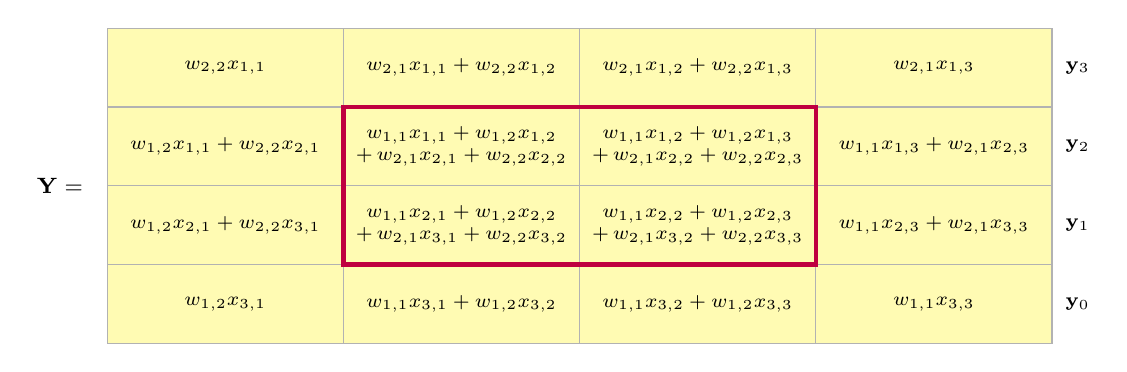
\begin{tikzpicture}[every node/.style={font=\scriptsize}]
    \node[font=\footnotesize] at (-0.6,2.0) {$\mathbf{Y} = $};
    \fill[yellow!30] (0,0) rectangle (12.0,4.0);
    \draw[gray!60, xstep=3.0, ystep=1.0] (0,0) grid (12.0,4.0);
    \draw[gray!60] (0,0) rectangle (12.0,4.0);
    % Miolo 2x2 = posicoes do modo valid
    \draw[ultra thick, purple] (3.0,1.0) rectangle (9.0,3.0);
    \node[align=center] at (1.5,3.5) {$w_{2,2}x_{1,1}$};
    \node[align=center] at (4.5,3.5) {$w_{2,1}x_{1,1} + w_{2,2}x_{1,2}$};
    \node[align=center] at (7.5,3.5) {$w_{2,1}x_{1,2} + w_{2,2}x_{1,3}$};
    \node[align=center] at (10.5,3.5) {$w_{2,1}x_{1,3}$};
    \node[align=center] at (1.5,2.5) {$w_{1,2}x_{1,1} + w_{2,2}x_{2,1}$};
    \node[align=center] at (4.5,2.5) {$w_{1,1}x_{1,1} + w_{1,2}x_{1,2}$\\$+\, w_{2,1}x_{2,1} + w_{2,2}x_{2,2}$};
    \node[align=center] at (7.5,2.5) {$w_{1,1}x_{1,2} + w_{1,2}x_{1,3}$\\$+\, w_{2,1}x_{2,2} + w_{2,2}x_{2,3}$};
    \node[align=center] at (10.5,2.5) {$w_{1,1}x_{1,3} + w_{2,1}x_{2,3}$};
    \node[align=center] at (1.5,1.5) {$w_{1,2}x_{2,1} + w_{2,2}x_{3,1}$};
    \node[align=center] at (4.5,1.5) {$w_{1,1}x_{2,1} + w_{1,2}x_{2,2}$\\$+\, w_{2,1}x_{3,1} + w_{2,2}x_{3,2}$};
    \node[align=center] at (7.5,1.5) {$w_{1,1}x_{2,2} + w_{1,2}x_{2,3}$\\$+\, w_{2,1}x_{3,2} + w_{2,2}x_{3,3}$};
    \node[align=center] at (10.5,1.5) {$w_{1,1}x_{2,3} + w_{2,1}x_{3,3}$};
    \node[align=center] at (1.5,0.5) {$w_{1,2}x_{3,1}$};
    \node[align=center] at (4.5,0.5) {$w_{1,1}x_{3,1} + w_{1,2}x_{3,2}$};
    \node[align=center] at (7.5,0.5) {$w_{1,1}x_{3,2} + w_{1,2}x_{3,3}$};
    \node[align=center] at (10.5,0.5) {$w_{1,1}x_{3,3}$};
    \foreach \k/\y in {3/3.5,2/2.5,1/1.5,0/0.5} \node[anchor=west] at (12.05,\y) {$\mathbf{y}_\k$};
\end{tikzpicture}
\vspace{0.3em}
\begin{itemize}
    \item Em destaque, as $2\times 2$ posições em que o filtro cabe inteiro dentro de $\mathbf{X}$ (modo \textit{valid}).
\end{itemize}
\end{frame}

\begin{frame}{\texttt{im2col} vs Versão Ingênua}
\begin{itemize}
    \item Versão ingênua em modo \textit{full}: deslizamos $\mathbf{\Theta}$ sobre $\mathbf{X}$ com \textit{padding} $K-1 = 1$ e preenchemos o \textit{feature map} posição a posição, $Y_{m,n} = \sum_{i,j} w_{i,j}\, x_{m+i-2,\, n+j-2}$.
\end{itemize}
\vspace{0.4em}
\centering
% Esquerda: X com padding (zeros em cinza, pixels em azul) e Theta; contorno laranja = janela
% da posicao calculada no passo. Direita: feature map Y, preenchido em ordem de varredura ate
% igualar o do Passo 9 (contorno roxo = celula do passo atual).
\begin{tikzpicture}[every node/.style={font=\scriptsize}]
    \begin{scope}[shift={(0,1.3)}, scale=0.52, every node/.style={font=\tiny}]
        \fill[gray!15] (0,0) rectangle (5,5);
        \fill[PastelBlue2!35] (1,1) rectangle (4,4);
        \draw[step=1, gray!60] (0,0) grid (5,5);
        \draw[gray!60] (0,0) rectangle (5,5);
        \node at (0.5,4.5) {$0$};
            \node at (1.5,4.5) {$0$};
            \node at (2.5,4.5) {$0$};
            \node at (3.5,4.5) {$0$};
            \node at (4.5,4.5) {$0$};
            \node at (0.5,3.5) {$0$};
            \node at (1.5,3.5) {$x_{1,1}$};
            \node at (2.5,3.5) {$x_{1,2}$};
            \node at (3.5,3.5) {$x_{1,3}$};
            \node at (4.5,3.5) {$0$};
            \node at (0.5,2.5) {$0$};
            \node at (1.5,2.5) {$x_{2,1}$};
            \node at (2.5,2.5) {$x_{2,2}$};
            \node at (3.5,2.5) {$x_{2,3}$};
            \node at (4.5,2.5) {$0$};
            \node at (0.5,1.5) {$0$};
            \node at (1.5,1.5) {$x_{3,1}$};
            \node at (2.5,1.5) {$x_{3,2}$};
            \node at (3.5,1.5) {$x_{3,3}$};
            \node at (4.5,1.5) {$0$};
            \node at (0.5,0.5) {$0$};
            \node at (1.5,0.5) {$0$};
            \node at (2.5,0.5) {$0$};
            \node at (3.5,0.5) {$0$};
            \node at (4.5,0.5) {$0$};
        \node[anchor=south, font=\scriptsize] at (2.5,5.05) {$\mathbf{X}$ com \textit{padding}};
        \only<1>{\draw[ultra thick, orange!80!black] (0,3) rectangle (2,5);}
        \only<2>{\draw[ultra thick, orange!80!black] (1,3) rectangle (3,5);}
        \only<3>{\draw[ultra thick, orange!80!black] (1,2) rectangle (3,4);}
    \end{scope}
    \begin{scope}[shift={(0.78,0.0)}, scale=0.5, every node/.style={font=\tiny}]
        \fill[orange!40] (0,0) rectangle (2,2);
        \draw[step=1, gray!60] (0,0) grid (2,2);
        \draw[gray!60] (0,0) rectangle (2,2);
        \node at (0.5,1.5) {$w_{1,1}$}; \node at (1.5,1.5) {$w_{1,2}$};
        \node at (0.5,0.5) {$w_{2,1}$}; \node at (1.5,0.5) {$w_{2,2}$};
        \node[anchor=west, font=\scriptsize] at (2.1,1) {$\mathbf{\Theta}$};
    \end{scope}
    \draw[->, gray!70, thick] (2.8,2.1) -- (3.4,2.1);
    % Feature map Y 4x4
    \begin{scope}[shift={(3.6,0.3)}]
        \node[anchor=south, font=\scriptsize] at (5.3,3.65) {\textit{feature map} $\mathbf{Y}$};
        \only<1->{\fill[yellow!30] (0.00,2.7) rectangle (2.65,3.6); \node[align=center] at (1.325,3.15) {$w_{2,2}x_{1,1}$};}
        \only<2->{\fill[yellow!30] (2.65,2.7) rectangle (5.30,3.6); \node[align=center] at (3.975,3.15) {$w_{2,1}x_{1,1} + w_{2,2}x_{1,2}$};}
        \only<3->{\fill[yellow!30] (5.30,2.7) rectangle (7.95,3.6); \node[align=center] at (6.625,3.15) {$w_{2,1}x_{1,2} + w_{2,2}x_{1,3}$};}
        \only<3->{\fill[yellow!30] (7.95,2.7) rectangle (10.60,3.6); \node[align=center] at (9.275,3.15) {$w_{2,1}x_{1,3}$};}
        \only<3->{\fill[yellow!30] (0.00,1.8) rectangle (2.65,2.7); \node[align=center] at (1.325,2.25) {$w_{1,2}x_{1,1} + w_{2,2}x_{2,1}$};}
        \only<3->{\fill[yellow!30] (2.65,1.8) rectangle (5.30,2.7); \node[align=center] at (3.975,2.25) {$w_{1,1}x_{1,1} + w_{1,2}x_{1,2}$\\$+\, w_{2,1}x_{2,1} + w_{2,2}x_{2,2}$};}
        \only<4->{\fill[yellow!30] (5.30,1.8) rectangle (7.95,2.7); \node[align=center] at (6.625,2.25) {$w_{1,1}x_{1,2} + w_{1,2}x_{1,3}$\\$+\, w_{2,1}x_{2,2} + w_{2,2}x_{2,3}$};}
        \only<4->{\fill[yellow!30] (7.95,1.8) rectangle (10.60,2.7); \node[align=center] at (9.275,2.25) {$w_{1,1}x_{1,3} + w_{2,1}x_{2,3}$};}
        \only<4->{\fill[yellow!30] (0.00,0.9) rectangle (2.65,1.8); \node[align=center] at (1.325,1.35) {$w_{1,2}x_{2,1} + w_{2,2}x_{3,1}$};}
        \only<4->{\fill[yellow!30] (2.65,0.9) rectangle (5.30,1.8); \node[align=center] at (3.975,1.35) {$w_{1,1}x_{2,1} + w_{1,2}x_{2,2}$\\$+\, w_{2,1}x_{3,1} + w_{2,2}x_{3,2}$};}
        \only<4->{\fill[yellow!30] (5.30,0.9) rectangle (7.95,1.8); \node[align=center] at (6.625,1.35) {$w_{1,1}x_{2,2} + w_{1,2}x_{2,3}$\\$+\, w_{2,1}x_{3,2} + w_{2,2}x_{3,3}$};}
        \only<4->{\fill[yellow!30] (7.95,0.9) rectangle (10.60,1.8); \node[align=center] at (9.275,1.35) {$w_{1,1}x_{2,3} + w_{2,1}x_{3,3}$};}
        \only<4->{\fill[yellow!30] (0.00,0.0) rectangle (2.65,0.9); \node[align=center] at (1.325,0.45) {$w_{1,2}x_{3,1}$};}
        \only<4->{\fill[yellow!30] (2.65,0.0) rectangle (5.30,0.9); \node[align=center] at (3.975,0.45) {$w_{1,1}x_{3,1} + w_{1,2}x_{3,2}$};}
        \only<4->{\fill[yellow!30] (5.30,0.0) rectangle (7.95,0.9); \node[align=center] at (6.625,0.45) {$w_{1,1}x_{3,2} + w_{1,2}x_{3,3}$};}
        \only<4->{\fill[yellow!30] (7.95,0.0) rectangle (10.60,0.9); \node[align=center] at (9.275,0.45) {$w_{1,1}x_{3,3}$};}
        \draw[gray!60, xstep=2.65, ystep=0.9] (0,0) grid (10.6,3.6);
        \draw[gray!60] (0,0) rectangle (10.6,3.6);
        % Celula calculada no passo atual (celulas ja percorridas continuam preenchidas)
        \only<1>{\draw[ultra thick, purple] (0,2.7) rectangle (2.65,3.6);}
        \only<2>{\draw[ultra thick, purple] (2.65,2.7) rectangle (5.3,3.6);}
        \only<3>{\draw[ultra thick, purple] (2.65,1.8) rectangle (5.3,2.7);}
        \only<4>{\draw[ultra thick, purple] (2.65,0.9) rectangle (7.95,2.7);}
    \end{scope}
\end{tikzpicture}
\vspace{0.4em}
\begin{itemize}
    \visible<4>{\item O \textit{feature map} ficou idêntico ao resultado do \texttt{im2col} no Passo 9. Sem o \textit{padding}, o laço calcularia apenas o miolo destacado: o modo \textit{valid}.}
\end{itemize}
\end{frame}

\begin{frame}{Por que \texttt{im2col} é a escolha prática}
\begin{itemize}
    \item Reduz a convolução a uma multiplicação de matrizes (\texttt{GEMM}), o tipo de operação que GPUs e bibliotecas BLAS otimizam ao máximo.
    \item Permite usar a mesma rotina para qualquer combinação de \textit{kernel}, \textit{stride} e \textit{padding}, alterando apenas o layout dos dados.
    \item Custa memória extra para armazenar as ``cópias'' das janelas, mas o ganho em velocidade compensa em larga escala.
\end{itemize}
\end{frame}

%========================================================================
\section*{Referências e Leituras}
%========================================================================

\begin{frame}{Leituras Recomendadas}
\leiturasize
\sloppy
\begin{itemize}
    \item Capítulo 10 de \fullcite{prince2023understanding}, livro disponível em \href{https://udlbook.github.io/udlbook/}{\textit{udlbook.github.io/udlbook}}.
    \item Materiais que também serviram de base para a aula:
    \begin{itemize}
        \item \textit{Machine Learning} @ Berkeley.
        \item Convolução como multiplicação de matrizes: \url{https://github.com/alisaaalehi/convolution_as_multiplication}.
        \item Aritmética de convoluções (\textit{padding}, \textit{stride}, convolução transposta): \url{https://github.com/vdumoulin/conv_arithmetic}.
    \end{itemize}
\end{itemize}
\end{frame}

\begin{frame}[allowframebreaks]{Referências}
\sloppy
\printbibliography[heading=none]
\end{frame}

\end{document}
